\documentclass{tesisilkomugm}

%-----------------------------------------------------------------
%Disini awal masukan untuk data Skripsi (ISI SESUAI DENGAN DATA ANDA!)
%-----------------------------------------------------------------
%\titleeng{ENHANCING OF HAND GESTURE RECOGNITION FOR LOW-LIGHT ENVIRONMENT USING RETINEX}
\titleind{PERBAIKAN PENGENALAN GESTUR TANGAN TERHADAP KONDISI LINGKUNGAN BERINTENSITAS CAHAYA RENDAH MENGGUNAKAN RETINEX}	

\fullname{ANTHONIUS ADI NUGROHO}
\NIM{19/448690/PPA/05773}
\examdate{04 Mei 2020}
\degree{Sarjana Sains}
\yearsubmit{2020}
\firstsupervisor{Dr. Raden Sumiharto, S.Si., M.Kom.}
\firstexaminer{Penguji 1}
\secondexaminer{penguji 2}
\thirdexaminer{...}


\begin{document}
\cover%\titlepage

%\approvalpage
%\declarepage
%Setelah Anda selesai Ujian Akhir Tesis, scan halaman pengesahan yang telah ditandatangani dosen pembimbing dan penguji, scan juga halaman pernyataan yang telah Anda tandatangani. Selanjutnya simpan hasil scan tersebut dalam bentuk PDF dengan nama pengesahanskripsi.pdf dan pernyataan.pdf (file disimpan di folder yang sama dengan folder dimana file Skripsi.tex tersimpan)
%Hilangkan karakter % sebelum perintah "\approvalpagescan" dan "\declarepage" di bawah ini, dan tambahkan karakter % sebelum perintah "\approvalpage" di atas.
\approvalpagescan
%\declarepage



%-----------------------------------------------------------------
%Halaman Persembahan (ISI SESUAI DENGAN DATA ANDA!)
%-----------------------------------------------------------------
%\acknowledment
%-----------------------------------------------------------------
%-----------------------------------------------------------------


%-----------------------------------------------------------------
%Halaman Motto (ISI SESUAI DENGAN DATA ANDA!)
%-----------------------------------------------------------------
%\motto

%-----------------------------------------------------------------
%-----------------------------------------------------------------


%-----------------------------------------------------------------
%Disini awal masukan untuk Prakata (ISI SESUAI DENGAN DATA ANDA!)
%-----------------------------------------------------------------
%\preface
%-----------------------------------------------------------------
%-----------------------------------------------------------------


%-----------------------------------------------------------------
%Daftar Isi (TIDAK PERLU DIUBAH)
%-----------------------------------------------------------------
\newpage\phantomsection\addcontentsline{toc}{chapter}{DAFTAR ISI}
\makeatletter\renewcommand\l@chapter[2]{\ifnum \c@tocdepth >\z@\addpenalty\@secpenalty\addvspace{0em}\setlength\@tempdima{1.4em}\begingroup\parindent \z@ \rightskip \@pnumwidth\parfillskip -\@pnumwidth\leavevmode \bfseries\advance\leftskip\@tempdima\hskip -\leftskip#1\nobreak\ \leaders\hbox{$\m@th\mkern \@dotsep mu\hbox{.}\mkern \@dotsep mu$}\hfil\nobreak\hb@xt@\@pnumwidth{\hss #2}\par\endgroup\fi}\makeatother
\begin{singlespacing}\tableofcontents\end{singlespacing}
%-----------------------------------------------------------------
%-----------------------------------------------------------------

%-----------------------------------------------------------------
%Daftar Tabel (JIKA DIPERLUKAN, HAPUS KARAKTER % SEBELUM \newpage dan \begin)
%-----------------------------------------------------------------
\newpage\phantomsection\addcontentsline{toc}{chapter}{DAFTAR TABEL}
\begin{singlespacing}\listoftables\end{singlespacing} 
%-----------------------------------------------------------------
%-----------------------------------------------------------------

%-----------------------------------------------------------------
%Daftar Gambar (JIKA DIPERLUKAN, HAPUS KARAKTER % SEBELUM \newpage dan \begin)
%-----------------------------------------------------------------
\newpage\phantomsection\addcontentsline{toc}{chapter}{DAFTAR GAMBAR}
\begin{singlespacing}\listoffigures\end{singlespacing}
%-----------------------------------------------------------------
%-----------------------------------------------------------------


%-----------------------------------------------------------------
%Daftar Lambang (ISI SESUAI DENGAN DATA ANDA!)
%-----------------------------------------------------------------
%-----------------------------------------------------------------
%-----------------------------------------------------------------


%-----------------------------------------------------------------
%Disini awal masukan Intisari (ISI SESUAI DENGAN DATA ANDA!)
%-----------------------------------------------------------------
\begin{abstractind}
Bahasa isyarat adalah salah satu bentuk komunikasi non-verbal antar manusia yang memiliki makna tersendiri. \emph{American Sign Language}(ASL) merupakan bentuk dari bahasa isyarat tangan yang digunakan oleh penyandang disabilitas untuk berkomunikasi satu sama lain. Penggunaan bahasa isyarat membantu penyetaraan hak atas informasi yang diberikan. Perkembangan ilmu yang sangat maju membantu seseorang dapat memahami suatu bahasa isyarat tanpa harus mempelajari hal tersebut. Salah satu bagian disiplin ilmu tersebut adalah pengenalan gestur, dimana di dalamnya terdapat bahasa isyarat yang dapat diterjemahkan dengan bantuan kamera.

Kamera digunakan sebagai alat yang mengimitasi mata manusia dalam mengenali sebuah gestur. Proses pengenalan bahasa isyarat memiliki beberapa hal penting di dalamnya. Intensitas cahaya merupakan salah satu faktor penting dalam pengambilan sebuah citra yang ditangkap oleh kamera, dimana merupakan suatu tantangan tersendiri ketika informasi citra tidak dapat ditangkap dengan jelas yang menyebabkan penurunan performa. Permasalahan ini dapat diatasi dengan menggunakan teori \emph{Retinex} yang diambil dari kata retina dan cortex. \emph{Retinex} mampu meningkatkan tingkat kecerahan citra dengan cara layaknya mata manusia yang dapat melihat walaupun dalam ruangan minim cahaya. Citra yang telah dilakukan perbaikan kontras akan dilakukan deteksi tangan kemudian akan dikenali bahasa isyarat tersebut menggunakan teknik \emph{Convolution Neural Network}.

\textbf{\emph{Kata kunci - Retinex, Hand Gesture Recognition, Object Detection} }
\end{abstractind}
%-----------------------------------------------------------------
%-----------------------------------------------------------------

%-----------------------------------------------------------------
%Disini awal masukan untuk Abstract (ISI SESUAI DENGAN DATA ANDA!)
%-----------------------------------------------------------------
%\begin{abstracteng}
%Gestures are one of meaningful non-verbal communication among humans. American Sign Language(ASL) is an example hand gesture useful for communicating disability persons to others. Sign language helps people to get right about information provided. Rapid scientific progress can help people to recognize sign language without having to learn. It called gesture recognition, which contains sign languages that can be translated by using camera.

%The camera is used to be human eyes to recognize gestures. Process of recognizing gesture has several important things. Light intensity is most important thing when image is taken by the camera,  which is a challenge when an image information is unclear makes performance degradation. The solution of low-light environment can be handled by using retinex theory, it's taken from the words retina and cortex. Retinex can increase contrast level image like a human eyes can see in a low-light environment. After light-enhanced, hand will be detected and gesture of an image will be recognized by using convolutional neural network.

%\textbf{\emph{Keywords - Retinex, Hand Gesture Recognition, Object Detection} }
%\end{abstracteng}
%-----------------------------------------------------------------
%-----------------------------------------------------------------

%-----------------------------------------------------------------
%Disini awal masukan untuk Bab (ISI BAB I DAPAT DIEDIT DI FILE Bab1.tex,
%ISI BAB II DAPAT DIEDIT DI FILE Bab2.tex, dst...)
%-----------------------------------------------------------------
\chapter{PENDAHULUAN}
\section{Latar Belakang Masalah}
Disabilitas adalah kelompok masyarakat yang memiliki keterbatasan yang dapat menghambat partisipasi dan peran serta mereka dalam kehidupan bermasyarakat. Penyandang disabilitas memiliki berbagai kategori, yaitu disabilitas fisik, intelektual, mental dan sensorik.
menurut data dari kemenkes tahun 2015, presentase 3 teratas penyandang disabilitas di provinsi indonesia adalah 6.36\% kesulitan melihat, 3.76\% kesulitan berjalan dan 3.35\% kesulitan mendengar (Kemenkes., 2018). Pemerintah Indonesia telah menandatangani konvensi tentang Hak-Hak Penyandang Disabilitas pada tanggal 30 Maret 2007 di New York. Adanya penandatanganan tersebut menunjukan bangsa indonesia menghormati, melindungi, memenuhi dan memajukan hak-hak penyandang disabilitas. Untuk itu perlu adanya dukungan dari masyarakat dalam mewujudkanya. 

Bagi penyandang disabilitas, mereka memiliki hambatan akses dalam melakukan aktivitas sehari hari. Dengan adanya perkembangan pengetahuan dan teknologi, mereka mulai terbantu dan dapat melakukan aktivitas layaknya masyarakat pada umumnya.
Mulai banyak penyandang disabilitas yang melakukan mobilitas tinggi dengan kursi roda, mengakses informasi dengan adanya penerjemah bahasa. Dengan adanya hal tersebut, penyandang disabilitas mendapat tempat dan peranan yang sama dengan masyarakat lainnya.

Teknologi yang semakin dewasa membuat mobilitas penyandang disabilitas menjadi lebih tinggi. Kursi roda mungkin dapat digunakan untuk membantu penyandang bergerak dari suatu tempat ke tempat lain, namun bagi beberapa penyandang disabilitas tertentu yang tidak memiliki kemampuan normal pada kondisi tangan atau lumpuh sebagian tidak dapat menggunakan kursi roda tersebut. Alhasil perlu adanya orang lain untuk membantu menngerakan kursi roda tersebut. 

Teknologi komputer dan robotika saat ini memiliki peranan penting dalam membantu sebuah permasalahan dari mulai kegiatan industri hingga kegiatan masyarakat. (Posada-Gómez et al., 2007) Membuat kursi roda pintar dengan kontrol gestur tangan, namun pada penelitian tersebut memiliki kelemahan terhadap cahaya. Intensitas cahaya yang cenderung rendah membuat sistem tidak mampu mendeteksi kontrol dari gestur tangan, sehingga hanya dapat digunakan dalam keadaan cahaya yang cenderung terang. Penelitian tersebut menggunakan teknologi pemrosesan citra yang dikombinasikan dengan elektronika dan mekanika untuk pergerakan kursi roda.

Penelitian yang menggunakan variasi cahaya juga dilakukan oleh (Saputra., 2016) dengan variasi metode \textit{Retinex} dan variasi intensitas cahaya 439,75 lux, 273,25 lux, 150 lux dan 9 lux. Penelitian yang dilakukan untuk meningkatkan akurasi deteksi wajah menggunakan \textit{adaboost haar-like}. Hasil pengujian pada penelitian ini menghasilkan nilai akurasi dengan rata-rata tertinggi dari 10 kali uji 96,67\% pada kondisi 439,75 lux, 90,59\% pada kondisi 273,25 lux, 42,29\% pada kondisi 150 lux dan 0\% pada kondisi 9 lux.

Pemrosesan citra memiliki beberapa hal fundamental permasalahan diantaranya adalah proses perbaikan citra. Perbaikan citra digunakan untuk memperbaiki sebuah citra yang bermasalah agar informasi citra terlihat lebih jelas secara visual maupun perhitungan. Penggunaan \emph{image processing} sangat dibutuhkan untuk membantu menyelesaikan permasalahan dalam kehidupan sehari hari. Aplikasi dari implementasi \emph{image processing} beberapa diantaranya adalah pengenalan dan deteksi pada sebuah objek. Untuk menyelesaikan permasalahan tersebut perlu membuat sistem yang tahan terhadap kondisi cahaya berintensitas rendah.

Pengenalan dan deteksi sebuah objek memiliki ruang lingkup yang sangat luas untuk di kembangkan, pada penelitian ini berfokus pada gesture recognition.
Dalam pemrosesan citra algoritme pada gesture recognition dapat di implementasikan pada komunikasi non verbal ataupun suatu gerakan yang dapat membantu seseorang menyelesaikan permasalahan. Pola pada gesture dapat dikenali oleh seseorang dengan cara melihat gesture tersebut, hal yang sama terjadi pada kamera yang mengadopsi apa yang dilakukan mata manusia untuk mengenali sebuah objek. 
\emph{Hand gesture} salah satu contoh implementasi \emph{image processing} yang dapat dikembangkan untuk membantu seseorang menyelesaikan permasalahan dengan menggunakan gestur tangan. 

Salah satu faktor yang dapat menurunkan kualitas suatu citra yaitu pencahayaan dari sebuah citra, proses pengambilan citra dalam intensitas rendah akan menghasilkan citra yang buruk (Saputra., 2016).
Implementasi algoritme untuk meningkatkan kualitas citra terhadap kondisi cahaya merupakan permasalahan yang menarik untuk diteliti.
Kondisi cahaya pada image processing adalah sesuatu topik yang menantang dalam permasalahan \emph{image processing} dan \emph{computer vision} untuk meningkatkan visibilitas maupun kualitas yang lebih baik dari suatu citra. 
Beberapa penelitian terdahulu telah melakukan peningkatan algoritme pada kondisi cahaya yang minim untuk suatu citra (Loh et al., 2019). 
Berkembangnya algoritme dalam ruang lingkup kondisi cahaya yang minim bertujuan mendapatkan kualitas kontras yang lebih jelas untuk dapat dilakukan komputasi lebih lanjut.

\emph{Retinex} merupakan metode yang diusulkan oleh Land dengan memodelkan pencahayaan dan persepsi warna berdasarkan penglihatan mata manusia. Mata manusia dapat membedakan sebuah objek sekalipun dalam kondisi intensitas cahaya yang rendah. Metode \emph{Retinex} terus mengalami berbagai pengembangan dari \emph{Single Scale Retinex} hingga \emph{Multiscale Retinex} berupaya untuk memperoleh keseimbangan kontras dalam pencahayaan berintensitas rendah(Saputra., 2016).

Peningkatan kontras menjadi salah satu solusi untuk meningkatkan visibilitas dari sebuah citra. Penelitian ini menggunakan algoritme \emph{Multiscale Retinex Color Restoration} untuk meningkatkan kontras serta \emph{object detection} untuk melakukan segmentasi pada suatu citra, kemudian untuk melakukan pengenalan sebuah gesture yang telah dilakukan perbaikan kontras, akan dilanjutkan dengan metode \emph{Convolutional Neural Network}. 

Implementasi dari peningkatan kontras untuk pengenalan gestur tangan ini diharapkan dapat dibawa untuk menyelesaikan permasalahan pada sistem yang bergantung pada cahaya. Beberapa sistem yang dimaksud seperti kursi roda pintar, ataupun sistem lainnya seperti pengenalan wajah dan pengenalan gestur maupun pendeteksi suatu objek yang menggunakan kamera. 
\section{Rumusan Masalah}
Berdasarkan rumusan masalah yang telah dijelaskan sebelumnya, maka rumusan masalah pada penelitian ini adalah nilai akurasi dari deteksi wajah dengan intensitas cahaya 150 lux hanya mampu 42,39\%, sehingga deteksi dan pengenalan sebuah objek sangat dipengaruhi oleh cahaya. Intensitas cahaya yang semakin rendah menyebabkan penurunan akurasi suatu deteksi dan pengenalan. Hal tersebut dapat berdampak pada performa sebuah sistem yang semakin menurun. 
\section{Batasan Masalah}
Penelitian ini memiliki batasan masalah yang bertujuan untuk tidak memperluas pokok bahasan. Batasan masalah yang digunakan dalam penelitian ini adalah sebagai berkut:
\begin{enumerate}
\item Acuan dataset menggunakan \emph{American Sign Language}, dengan sepuluh klasifikasi yaitu angka 0 hingga angka 9.
\item Data yang digunakan menggunakan dataset private dan dataset public.
\item Proses pengujian akan dilakukan dengan 3 subjek dengan warna kulit yang berbeda.
\item Penurunan intensitas cahaya dikurangi sebesar 50\% lux sebelumnya hingga nilai lux kurang dari 50 lux.
\end{enumerate}
\section{Tujuan Penelitian}
Penelitian yang dilakukan bertujuan untuk mengatasi permasalahan sistem yang bergantung pada pencahayaan dengan mengimplementasikan algoritme \emph{Retinex} pada sebuah sistem deteksi dan pengenalan gestur tangan, dengan tingkat intensitas cahaya yang bervariasi.
\section{Manfaat Penelitian}
Penelitian ini diharapkan dapat memberi manfaat berupa:
\begin{enumerate}
\item Memberikan fitur tambahan untuk sistem yang memiliki permasalahan dengan pencahayaan dalam intensitas cahaya rendah.
\item Meningkatkan akurasi pengenalan gestur tangan dan deteksi objek pada kondisi cahaya berintensitas rendah.
\end{enumerate}



\chapter{TINJAUAN PUSTAKA} 
Penelitian untuk menghasilkan algoritme deteksi dan pengenalan gestur sudah banyak dilakukan, sehingga banyak metode yang memiliki tingkat keberhasilan tinggi. Namun pada pemrosesan citra tingkat keberhasilan tidak hanya didukung pada algoritme deteksi dan pengenalan saja, namun kualitas pada citra tersebut harus memiliki kualitas yang bagus pula sehingga dapat menghasilkan akurasi yang tinggi(Saputra., 2016).

Salah satu hal yang mempengaruhi kualitas tersebut adalah kondisi cahaya yang mengarah pada objek, sehingga mempengaruhi hasil yang ditangkap oleh kamera. Peningkatan kontras sangat dibutuhkan untuk meningkatkan kualitas image dalam kondisi cahaya yang minim. Salah satu pendekatan yang populer dipakai adalah Retinex. (Tanaka et al., 2019) mengimplementasikan Retinex pada prepocessing untuk meningkatkan kontras citra. Percobaan yang dilakukan dengan membandingkan hasil segmentasi citra asli dan citra dengan proses preprocessing. Hasil yang didapat secara kualitatif terlihat setelah dilakukan segmentasi Gaussian Mixture Model. Hasil segmentasi objek dengan citra preprocessing mendapatkan foreground yang jelas daripada citra asli. Namun pada citra dengan Retinex peningkatan kontras berubah menghasilkan warna yang tidak natural.

Peningkatkan pencahayaan pada citra dapat dilakukan dengan banyak metode. Selain Retinex, metode yang paling populer adalah \emph{Histogram Equalization}. (Srinivasan, 2016) Melakukan perbandaingan antara algoritme \emph{Retinex} dan \emph{Histogram Equalization}. Pada penelitian tersebut \emph{Retinex} yang di implementasikan adalah \emph{Single Scale Retinex} (SSR) dan \emph{Multiscale Retinex} (MSR). Kemudian \emph{Histogram Equalization} yang diimplementasikan adalah BBHE, DSIHE dan RLBHE Kedua algoritme tersebut diuji menggunakan citra yang sama kemudian dilakukan perbandingan. 

Pada citra keluaran \emph{Histogram Equalization} (BBHE dan DSIE), citra mengalami meningkatkan kontras dengan keterbatasan beberapa fitur yang tidak terlihat, Keluaran RLBHE mereduksi kualitas dari piksel. Kemudian dengan citra keluaran \emph{Retinex}, citra mengalami peningkatan kontras dengan fitur yang terlihat lebih jelas daripada citra \emph{Histogram Equalization}.

Algoritme Retinex telah mengalami pengembangan untuk meningkatkan kualitas citra pada kondisi lingkungan tertentu. Saputra ditahun 2016 melakukan perbandingan variasi Retinex untuk peningkatan deteksi wajah yang dilakukan pada kondisi ruangan berintensitas rendah. Algoritme \emph{Adaptive Multiscale Retinex} (AMSR), \emph{Multiscale Retinex Color Restoration}(MSRCR) di implementasikan pada 4 kondisi cahaya. Hasil peningkatan maksimal yang didapatkan pada MSRCR dapat meningkatkan 1.46 kali dan ASMR mampu meningkatkan 1.11 kali. Namun peningkatan tersebut terjadi pada parameter intensitas 273.25 lux(Saputra., 2016).

Pengembangan MSR juga dilakukan oleh (Shen et al., 2017) dengan menambah layer preprocessing/post processing pada proses konvolusi citra pada CNN menjadi MSR-Net. Kemudian dibandingkan dengan MSRCR dan beberapa metode lainnya.  
Hasil MSR-Net mengalami peningkatan kontras citra dengan warna natural dibandingkan MSRCR dan beberapa metode lainnya.

Pengenalan sebuah gestur adalah yang menentukan hasil akhir dari sistem. CNN merupakan salah satu algoritme yang sering dijadikan solusi untuk proses klasifikasi dalam \emph{machine learning}. Beberapa penelitian menggunakan CNN dengan beberapa variasi parameter. Penelitian (Yingxin et al., 2017) menggunakan CNN untuk mengenali sebuah gestur tangan dengan dataset \emph{Cambridge hand gesture datasets} (CHGD). Pada penelitian ini dilakukan parameter illuminasi cahaya pada beberapa kondisi. Pengenalan gestur menghasilkan angka presentase yang tinggi sebesar 94.1\%. Proses dalam preprocessing menggunakan \emph{canny edge} untuk menghilangkan efek illuminasi. \emph{Canny edge} sangat membantu untuk kondisi illuminasi cahaya dibandingkan dengan algoritme CNN saja yang menggunakan citra asli di dapat hasil 70.0\%.

Pada citra gelap informasi atau fitur fitur penting dari sebuah citra akan tersembunyi. Informasi dalam sebuah citra penting untuk merepresentasikan sebuah citra itu sendiri. Untuk mendapatkan informasi tersebut pada penelitian (Loh et al., 2019) berfokus pada perbaikan citra dengan tujuan memperoleh fitur untuk mendukung sistem visi otomatis dimana sebuah citra memiliki kontras dan pencahayaan yang rendah. Dalam penelitian ini memodelkan sebuah citra dengan cahaya rendah sebagai distribusi peningkatan fungsi lokal menggunakan proses gaussian yang dilatih pada saat runtime menggunakan data referensi yang dihasilkan dari sebuah CNN. CNN sendiri dilatih menggunakan dengan data yang sangat besar berdasarkan statistik pencahayaan. Sehingga proses pembelajaran dapat mempelajari hubungan antara fitur dengan piksel. Dengan demikian refrensi  yang dihasilkan melatih gaussian proses untuk melakukan representasi fitur dengan benar. 

Dasar-dasar penelitian sebelumnya yang menjadi tinjauan pustaka pada penelitian ini dirangkum dalam Tabel 2.1. 

\begin{table}[htbp]
	\caption{Tinjauan Pustaka}
	\label{labelku}
	\vspace{0.2cm}
	
	\begin{tabular}{|p{0.5cm}|p{2cm}|p{3cm}|p{3cm}|p{4cm}|}
		\hline
		No \centering & Nama \centering &\centering  Penelitian & \centering Metode & \ \ \ \ \ \ \ \ \  \ \ \ \ Hasil \\
		
		\hline
		1 & (Loh et al., 2019) & \emph{Low-light image enhancement using Gaussian Process for features retrieval} & \emph{Gaussian process and Convolutional Neural Network} & Citra dengan kontras yang sangat rendah dapat di perbaiki menggunakan gaussian prosses dan CNN untuk memperoleh detail informasi dari sebuah objek \\
		
		\hline
		2 & (Tanaka et al., 2019) & \emph{Retinex Foreground Segmentation for Low Light Environments} & \emph{Retinex} dan \emph{Gaussian Mixture Model} & Secara kualitatif citra yang dihasilkan setelah melalui \emph{preprocessing} algoritme Retinex dapat meningkatkan pencahayaan dari sebuah citra\\
		
		\hline
		3 & (Yingxin et al., 2017) & \emph{A Robust Hand Gesture Recognition Method via Convolutional Neural Network} & \emph{Edge detection} dan \emph{Convolutional Neural Network} & Pengenalan gestur tangan mendapatkan hasil 94.1\% digabungkan dengan proses deteksi tepi.\\
		\hline
	\end{tabular}
\end{table}

\begin{table}[htpb]
	\caption{Lanjutan Tabel}
	\label{labelku}
	\vspace{0.2cm}
	\begin{tabular}{|p{0.5cm}|p{2cm}|p{3cm}|p{3cm}|p{4cm}|}
		\hline
		4 & (Shen et al., 2017) & \emph{MSR-Net:Low-light Image Enhancement using Deep Convolutional Network} & MSR-net & Hasil dari implementasi algoritme MSR-Net di bandingkan dengan MSRCR dan beberapa algoritme lain mendapatkan kontras yang lebih tinggi dengan warna yang natural dibandingkan algoritme lain.\\
		\hline
		5 & (Saputra., 2016) & Perbandingan Varian \emph{Metode Multiscale Retinex} Untuk Peningkatan Akurasi Deteksi Wajah \emph{Adaboost HAAR-like} & Variasi metode \emph{Multiscale Retinex} & Kondisi 439.75 lux MSRCR meningkatkan akurasi 1.31 kali dan
		AMSR hanya 1,11 kali.
		Kondisi 273.25 lux MSRCR 1.46 kali dan AMSR 1.31 kali.
		Kondisi 150 lux 
		MSRCR 1.38 kali dan AMSR 0.97 kali. 
		Kondisi 9 lux kedua algoritme tidak dapat mendeteksi wajah sebuah citra.\\
		\hline	
		
		6 & (Srinivasan, 2014) & Perbandingan antara \emph{Retinex} dan \emph{Histogram Equalization} & SSR, MSR, BBHE, DSIHE, RLBHE & Citra keluaran \emph{Retinex} memiliki \emph{output} kontras yang baik tanpa menghilangkan fitur pada citra. \\
		\hline	
		7 & (Arabi, 2019) & Mendeteksi peralatan konstruksi yang diaplikasikan pada embedded system dan PC & \emph{SSD MobileNet} & Untuk semua device mAP $>$ 90\% \\
		\hline
		8& (Huang et al., 2019) &\emph{Hand Gesture Recognition with Skin Detection and Deep Learning Method Hand Gesture Recognition with Skin Detection and Deep Learning Method}& \emph{Skin detection} dan \emph{Convolutional Neural Network} & Menghasilkan akurasi 98.41\% \\
		\hline
	\end{tabular}
\end{table}

\chapter{LANDASAN TEORI}
\section{Computer Vision}
\emph{Computer vision} adalah teknologi yang membuat computer dapat melihat layaknya mata manusia. Penggunaan computer vision tanpa kita sadari telah di implementasikan dalam membantu menyelesaikan persoalan sehari hari. Contoh implementasi \emph{computer vision} antara lain \emph{face recognition, object classification, medical imaging,gesture recognition, video surveillance , 3D reconstruction}. Pada pengolahan citra, sebuah citra memiliki fitur fitur dari penting yang digunakan sebagai informasi saat pengolahan. Namun untuk mendapatkan suatu hasil, beberapa tahap proses harus dilakukan seperti \emph{preprocessing}, ekstraksi ciri, \emph{post-processing} dan sebagainya.
\section{Citra Digital}
Citra dapat didefinisikan sebagai fungsi \(f(x,y)\) berukuran \(M\) baris dan \(N\) kolom, dengan \(x\)  dan \(y\) adalah koordinat spasial dan amplitudo \(f\)  di titik koordinat \((x,y)\) dinamakan tingkat keabuan dari suatu citra. Apabila nilai \((x,y)\) dan \(f\) secara keseluruhan berhingga dan bernilai diskrit maka citra tersebut adalah citra digital. Citra digital dalam bentuk matrik dapat dilihat pada Persamaan 3.1 dan posisi koordinat citra digital dapat dilihat pada gambar 3.1(Sarifudin.,2015).

% TODO: \usepackage{graphicx} required
\begin{figure}[H]
	\centering
	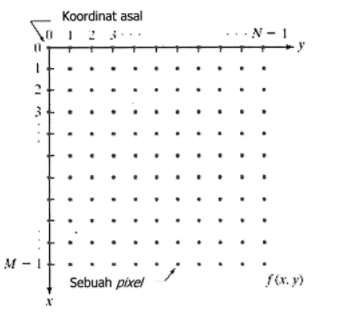
\includegraphics[width=0.3\linewidth]{screenshot001}
	\caption{Koordinat Citra Digital (Sarifudin.,2015)}
	\label{fig:screenshot001}
\end{figure}
\begin{equation}
f(x,y)
\begin{bmatrix}
f(0,0) & f(0,1) & ... & f(0,n-1)\\
f(1,0) & f(1,1) & ... & f(1,n-1)\\
... & ... & ... & ...\\
f(m-1,0) & f(m-1,1) & ... & f(m-1,n-1)\\
\end{bmatrix}
\end{equation}

\subsection{Citra RGB}
Citra RGB disebut juga sebagai citra berwarna, citra ini menyajikan tiga layer warna yaitu Red, Green dan Blue. Setiap piksel dari citra RGB merupakan gabungan dari variasi nilai intensitas tiga warna dasar yaitu merah(R), hijau(G), biru(B). Tiga warna tersebut dikodekan dengan 8 bit,dengan total ketiganya 3 x 8 = 24 bit. Sehingga variasi warna sebanyak $2^{24}$ = 16.777.216 variasi warna (Sarifudin., 2015). Contoh citra RGB dapat dilihat pada Gambar 3.2.
% TODO: \usepackage{graphicx} required
\begin{figure}[H]
	\centering
	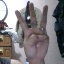
\includegraphics[width=0.35\linewidth]{29}
	\caption{Citra RGB}
	\label{fig:29}
\end{figure}

\subsection{Citra HSV}
Ruang warna HSV memiliki tiga komponen warna, yaitu Hue(H), Saturation(S) dan Value(V).
Hue memiliki variasi warna yang digambarkan secara melingkar, dimana merepresentasikan warna dari merah, kuning, hijau, cyan, biru, magenta,dan kembali lagi ke merah.
Saturation memiliki variasi nilai 0 hingga 1, dimana merepresentasikan saturasi warna dari merah ke merah muda dan Value memiliki nilai 0 hingga 1 yang merepresentasikan intensitas warna atau tingkat kecerahan dari hitam ke putih, dimana nilai semakin tinggi semakin cerah (Kolkur et al., 2017).
Ruang warna HSV dapat di gambarkan seperti Gambar 3.3.
% TODO: \usepackage{graphicx} required
\begin{figure}
	\centering
	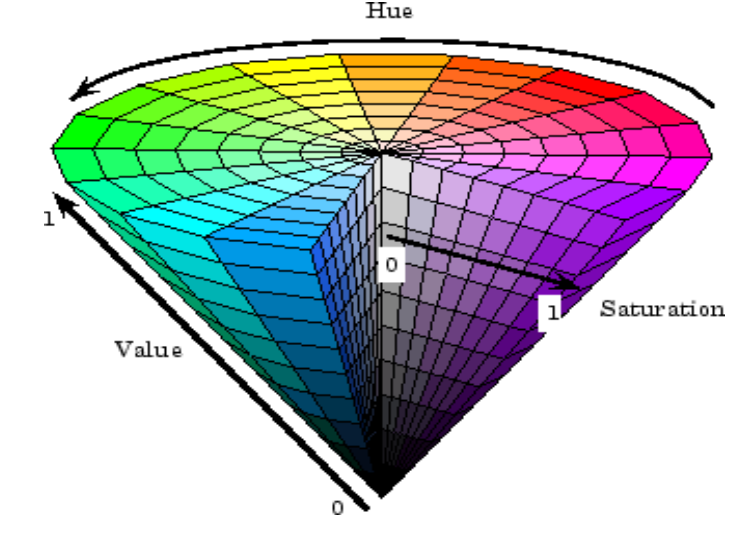
\includegraphics[width=0.45\linewidth]{hsv}
	\caption{Ruang warna HSV (Kolkur et al., 2017)}
	\label{fig:hsv}
\end{figure}

Pada RGB suatu warna di representasikan dengan nilai tiap komponen, namun untuk ruang warna HSV memiliki nilai yang berbeda dari RGB. Hue memiliki range dari 0$^\circ$ sampai 360$^\circ$. Transformasi warna dari RGB ke HSV dapat dilihat dalam Persamaan 3.2, 3.3, 3.4, 3.5.
\begin{equation}
	V = max(R,G,B)
\end{equation}
\begin{equation}
	S=
	\begin{cases}
	\frac{max(R,G,B) - min(R,G,B)}{max(R,G,B)} &  V \ne 0\\
	0 & lainnya
	\end{cases} 	
\end{equation}
\begin{equation}
	H=
	\begin{cases}
	\frac{60(G-B)}{V-min(R,G,B)} &  V=R \\
	120+\frac{60(B-R)}{V-min(R,G,B)} &  V=G \\
	240+\frac{60(R-G)}{V-min(R,G,B)} &  V=B \\
	\end{cases}
\end{equation}
\begin{equation}
	H = H+360
\end{equation}
Penggunaan citra dengan ruang HSV mampu memisahkan informasi warna sesuai dengan kemampuan mata manusia(Afrianto \& Amalia., 2016).
%=====================================operasi morfologi=======================================
\section{Operasi Morfologi}
\subsection{Erosi}
Operasi erosi adalah operasi penipisan objek yang terdapat pada citra biner. Operasi erosi dilakukan dengan cara mengurangi piksel pada kontir dari objek citra sesuai dengan kernel. Operasi erosi dinotasikan pada Persamaan 3.6 (Hidayatullah., 2017).
\begin{equation}
A \ominus B = A^c \oplus B^c
\end{equation}
\subsection{Dilasi}
Operasi dilasi adalah operasi penebalan  objek yang terdapat pada citra biner. Operasi ini dilakukan dengan menambah piksel pada kontur dari objek sesuai dengan kernel. Operasi ini berguna untuk menghaluskan citra dan menutupi lubang-lubang yang kosong. Operasi dilasi dinotasikan pada Persamaan 3.7 (Hidayatullah., 2017).
\begin{equation}
A \oplus B = t \ \epsilon \ Z^2 : t = a + b, a \ \epsilon \ A, \ b \ \epsilon \ B
\end{equation}

\subsection{\emph{Opening}}
Operasi \emph{opening} merupakan operasi yang biasa digunakan untuk memperhalus kontur citra serta menghilangkan lubang-lubang kecil pada citra. Operasi ini terdiri dari 2 dua tahap yaitu erosi kemudian dilanjutkan dilasi. Operasi erosi berguna untuk menghilangkan noise pada citra karena struktur latar depan yang berukuran kecil tereliminasi, sedangkan dilasi digunakan untuk menebalkan citra. Operasi opening dinotasikan dalam Persamaan 3.8(Hidayatullah., 2017).
\begin{equation}
A \bullet B = (A \ominus B) \oplus B
\end{equation}

\subsection{\emph{Closing}}
Operasi \emph{closing} merupakan kebalikan dari operasi \emph{opening}. Terdiri dari dua tahap yaitu operasi dilasi kemudian dilanjutkan dengan operasi erosi. Kegunaan operasi ini adalah untuk menutupi lubang yang kosong pada citra dengan menggunakan dilasi kemudian dilakukan erosi citra untuk menipiskan suatu citra. Operasi closing dinotasikan pada Persamaan 3.9 (Hidayatullah., 2017).
\begin{equation}
A \bullet B = (A \oplus B) \ominus B
\end{equation}
%=====================================end of operasi morfologi=================================
\section{\emph{Hand Gesture Recognition}}

\subsection{\emph{American Sign Language}(ASL)}
Bahasa isyarat merupakan media komunikasi utama bagi kaum difabel khusunya penyandang tunarungu di dunia. Setiap negara mempunyai bahasa isyarat masing masing. Dengan adanya bahasa isyarat, penyandang tunarungu dapat melakukan komunikasi antar sesama penderita maupun berkomunikasi dengan setiap orang. Bahasa isyarat mulai banyak digunakan pada siaran televisi, seperti acara debat ataupun channel berita dengan dibantu penerjemah bahasa isyarat. Dengan begitu memberi mereka hak yang sama untuk mendapatkan informasi. 

Salah satu bahasa isyarat yang digunakan adalah \emph{American Sign Language}(ASL). \emph{American Sign Language} menjadi salah satu alat bantu pembelajaran komunikasi untuk penggunanya. penggunaan bahasa isyarat dilakukan dengan gerakan gestur tangan yang memiliki makna untuk setiap pose. Pada penelitian ini, bahasa isyarat yang digunakan untuk menguji sistem adalah \emph{American Sign Language}. Pada gestur ASL, mempunyai beberapa bentuk gestur tangan huruf dan angka seperti pada Gambar 3.4.
% TODO: \usepackage{graphicx} required
\begin{figure}[H]
	\centering
	\includegraphics[width=0.7\linewidth]{"asl"}
	\caption{American Sign Language (Barczak et al., 2011)}
	\label{fig:asl}
\end{figure}
%!=============================================== Retinex
\section{Retinex(Single Scale Retinex)}
Algoritme \emph{Retinex} merupakan algoritme yang berusaha untuk mempertahankan ketetapan warna dimana warna suatu objek yang dilihat dalam keadaan pencahayaan yang berbeda(Aribowo et al., 2009). Algoritme \emph{Retinex} ini sering juga disebut dengan \emph{Single Scale Retinex} (SSR) karena hanya memiliki satu kanal. Menurut Land sebuah citra terbentuk sebagai perkalian reflektansi dan iluminasi. Berdasarkan teori \emph{Retinex} dapat dituliskan secara matematis seperti Persamaan 3.10 berikut(Parihar \& Singh., 2018)(Petro et al., 2014):
\begin{equation}
	I(x,y) = L(x,y) \boldsymbol{\cdot} R(x,y)
\end{equation}
\begin{equation}
	\log I(x,y) = \log L(x,y) + \log R(x,y)
\end{equation}
\begin{equation}
	\log R(x,y) = \log I(x,y)-\log L(x,y)
\end{equation}
dimana
\begin{equation}
	L(x,y)=F(x,y) * I(x,y)
\end{equation}
\begin{equation}
F(x,y) = \frac{1}{2\pi \sigma^2}e^{-(\frac{x^2 + y^2}{2\sigma^2})}
\end{equation}
\begin{equation}
	\int F(x,y) dxdy = 1
\end{equation}
sehingga
\begin{equation}
\log R = \log I(x,y) - \log [F(x,y) * I(x,y)]
\end{equation}
Keterangan :\\
\(I(x,y) \ :\) representasi dari kumpulansinyal dari citra asli.\\
\(R(x,y) :\) representasi dari komponen reflektansi dari objek.\\
\(L(x,y) :\) representasi komponen pencahayaan yang memenuhi Persamaan 3.12.\\
\(F(x,y) : \) \emph{gaussian function} yang memenuhi Persamaan 3.13.

Bentuk logaritmik pada Persamaan 3.11 digunakan untuk memisahkan antara komponen pencahayaan dan komponen reflektansinya. Pemisahan ini dilakukan untuk mendapatkan informasi dari citra tersebut sehingga hasil \emph{Single Scale Retinex} dapat dilihat pada Persamaan 3.17, dimana $\log R =$ \(R_{SSRi}\) adalah hasil \emph{Single Scale Retinex} pada kanal \(i\) (Parihar \& Singh., 2018)(Petro et al., 2014).
\begin{equation}
\centering
R_{SSRi}(x,y) = \log I_i(x,y) - \log [F(x,y) * I_i(x,y)]
\end{equation}
%!=============================================== MSR==============================
\subsection{Multiscale Retinex(MSR)}
\emph{Multiscale Retinex} merupakan pengembangan dari \emph{Single Scale Retinex} dengan menggabungkan beberapa scale  yang berbeda dengan pembobotan tertentu, dimana bobot tersebut jika dijumlahkan menghasilkan nilai 1. Sehingga nilai  sangat mempengaruhi detail warna dari sebuah citra. Bentuk matematis dari \emph{multiscale Retinex} dapat dilihat pada Persamaa 3.15 dan 3.16 berikut(Petro et al., 2014):
\begin{equation}
R_{MSRi} = \sum_{n=1}^{N} \omega_n R_{SSRi}=\omega_n [\log I(x,y) - \log (F_n(x,y) * I_i(x,y))]
\end{equation}
Keterangan :
\\
\(R_{MSRi} : \) hasil \emph{Multiscale Retinex} pada kanal i
\\
\(\omega_n \ \ \ \ \ \ \ : \) bobot pada skala n\\
Pada SSR dapat menyediakan kompresi rentang dinamis dan penampakan warna, namun keduanya tidak secara bersamaan. Oleh karena itu \emph{Multiscale Retinex} menggabungkan kompresi rentang dinamis dari \emph{Single Scale Retinex} dengan penampakan warna(Aribowo et al., 2009).
%!=============================================== MSRCR
\subsection{Multiscale Retinex Color Restoration(MSRCR)}
MSRCR merupakan pengembangan dari metode MSR yang mampu memperbaiki kualitas citra yang berhubungan dengan pencahayaan yaitu dengan mempertahankan \emph{color constancy}. \emph{Color constancy} berfungsi untuk mempertahankan komposisi warna suatu citra tetap terlihat sama walaupun kondisi pencahayaan yang berbeda-beda (Saputra., 2016). Perhitungan MSRCR dapat dilihat pada Persamaan 3.19, 3.20, 3.21 dan 3.22(Petro et al., 2014).
\begin{equation}
	R'_{MSRCRi}(x,y) = C_i(x,y) \ R_{MSR_i}(x,y)	
\end{equation}
\begin{equation}
	C_i(x,y) = \beta \ {\log[\alpha I'_i(x,y)]}\\
\end{equation}
\begin{equation}
I'(x,y) =\frac{I_i(x,y)}{\sum_{i=0}^{S}I_i(x,y)}
\end{equation}
\begin{equation}
	R_{MSRCRi}(x,y) = G \ [R'_{MSRCRi}(x,y)-b]
\end{equation}
\noindent Keterangan :\\
$i$ = 3 kanal warna RGB\\
$\alpha$ = konstanta kontrol ketidaklinieran\\
$\beta$ = konstanta gain\\
$G$,$b$ = gain dan offset
%!=============================================== MOBILENET
\section{MobileNet}
\emph{MobileNet} merupakan salah satu arsitektur CNN yang dibangun oleh \emph{Google} dan dikhususkan untuk \emph{mobile device} karena proses komputasi yang ringan. Perbedaan arsitektur \emph{MobileNet} dan CNN pada umumnya terdapat pada penggunaan layer konvolusi dengan ketebalan sesuai input dari citra. Arsitektur SSD \emph{MobileNet} menggunakan \emph{Depthwise layer} dan \emph{Pointwise layer}.
\subsection{Depthwise Separable Convolution}
\emph{Depthwise separable convolution} merupakan kunci utama untuk membangun arsitektur \emph{neural network}. Ide utamanya adalah mengganti operator konvolusi secara menyeluruh dengan memisahkan konvolusi menjadi dua lapisan terpisah. Layer pertama adalah \emph{depthwise convolution}, layer ini memiliki \emph{light-weight filter} dengan menggunakan \emph{single convolutional filter} untuk setiap input channel. Layer kedua menggunakan 1x1 convolution yang disebut dengan \emph{pointwise convolution} dimana layer ini membentuk fitur fitur baru melalui perhitungan kombinasi linear dari input channel. 

Pada konvolusi biasa memiliki input citra $D_F$ x $D_F$ x $M $ fitur map pada $F$ dan menghasilkan $ D_G$ x $D_G$ x $N $ fitur map pada $G$, dimana $D_F$ adalah tinggi dan lebar dari fitur map. $M$ merupakan jumlah input channel(input depth). 
$D_G$ merupakan tinggi dan lebar keluaran fitur map dan $N$ adalah keluaran channel dari fitur map\emph{(output depth)}. Kemudian kernel pada konvolusi biasa $D_K$ x $D_K$ x $M$ x $N$, dimana $D_K$ adalah dimensi kernel, $M$ jumlah input channel dan $N$ jumlah keluaran channel. Total cost dari konvolusi biasa memiliki ketergantungan pada $M$ pada Persamaan 3.23.
\begin{equation}
	D_K \bullet D_K \bullet M \bullet N \bullet D_F \bullet D_F
\end{equation}

\emph{Depthwise separable convolution} terbentuk dari layer \emph{depthwise convolution} dan \emph{pointwise convolution}. \emph{Depthwise convolution} sangat efisien daripada konvolusi biasa, namun pada layer \emph{depthwise} tersebut tidak menghasilkan fitur baru, oleh karena itu digunakan tambahan layer \emph{pointwise convolution} untuk menghitung linier kombinasi dari keluaran \emph{depthwise convolution} menggunakan 1x1 \emph{convolutio}n ,sehingga menghasilkan fitur baru. Total cost dari \emph{depthwise convolution} pada Persamaan 3.24.
\begin{equation}
D_K \bullet D_K \bullet M \bullet D_F \bullet D_F
\end{equation}
Kombinasi kedua layer tersebut dinamakan \emph{deptwise separable convolution} yang memiliki total cost Persamaan 3.25 :
\begin{equation}
D_K \bullet D_K \bullet M \bullet N \bullet D_F \bullet D_F + M \bullet N \bullet D_F \bullet D_F
\end{equation}
\emph{MobileNet} menggunakan 3x3 \emph{depthwise separable convolution} yang mana mereduksi komputasi 8 hingga 9 kali lebih cepat dari konvolusi biasa. Perbedaan konvolusi biasa dan \emph{depthwise separable convolution} digambarkan pada Gambar 3.5(Howard et al., 2017).
% TODO: \usepackage{graphicx} required
\begin{figure}[H]
	\centering
	\includegraphics[width=0.5\linewidth]{"new"}
	\caption{Convolutional standard dan depthwise separable (Howard et al., 2017)}
	\label{fig:new}
\end{figure} 
%!=============================================== MOBILENETV2 
\section{MobileNetV2}
Perbedaan \emph{MobileNet} versi kedua merupakan pengembangan dari \emph{MobileNet} versi pertama. Pada \emph{MobileNet} memiliki modifikasi arsitektur linier \emph{bottleneck} dan \emph{shortcut} koneksi antar \emph{bottleneck} seperti Gambar 3.6.
Sehingga arsitektur dalam \emph{MobileNetV2} menjadi \emph{bottleneck depth-separable convolution residuals}. Arsitektur \emph{bottleneck} dituliskan pada Tabel 3.1.
\begin{table}[H]
	\caption{Blok Arsitektur \emph{Bottleneck MobileNetV2} (Sandler et al., 2018)}
	\vspace{0cm}
	\centering
	\begin{tabular}{|p{3cm}|p{4cm}|p{3cm}|}
		\hline
		Input & Operator & Output \\
		\hline
		$h \ x \ w \ x \ k$ & 1$x$1 Conv2D, ReLU6 & $h \ x \ w$ (tk) \\ 
		\hline	
		$h \ x \ w \ x \ tk$ & 3$x$3 dwise s=s, ReLU6 & $\frac{h}{s} \ x \ \frac{w}{s}$ (tk) \\ 
		\hline	
		$\frac{h}{s} \ x \ \frac{w}{s} \ x \ tk$ & linear 1$x$1 Conv2D & $\frac{h}{s} \ x \ \frac{w}{s}$ k' \\ 
		\hline				
	\end{tabular}
\end{table}
Tabel 3.1 menunjukan blok arsitektur \emph{bottleneck} \emph{MobileNetV2} terdiri dari \emph{fully convolution} dengan 32 filter diikuti 19 layer \emph{residual bottleneck}.
Kernel yang digunakan menggunaka ukuran 3x3 (standard untuk modern network) dan menggunakan dropout dan normalisasi selama pelatihan(Sandler et al., 2018). 
\begin{figure}[H]
	\centering
	\includegraphics[width=0.6\linewidth]{"arsitektur"}
	\caption{Struktur Dasar Pada \emph{MobileNetV2} (Google AI Blog., 2018)}
	\label{fig:arsitektur}
\end{figure}
\noindent Pada bagian \emph{bottleneck} terdapat \emph{input} dan \emph{output}, sedangkan layer di bagian dalam mengenkapsulasi kemampuan model untuk merubah input dari piksel ke gambar. Tambahan \emph{shortcut} antar \emph{bottleneck} memungkinkan saat melakukan \emph{training} menjadi lebih cepat dengan peningkatan akurasi yang lebih baik(Google AI Blog,. 2018).
%!=============================================== ConvNeuralNet
\section{Convolutional Neural Network(CNN)}
\emph{Convolutional Neural Network} (CNN) merupakan jaringan syaraf tiruan yang memiliki arsitektur khusus yang dapat bekerja dengan baik dalam penggunaannya pada pemrosesan data berbentuk larik, seperti data runtun waktu dan citra digital. Dalam arsitekturnya CNN menggunakan operasi matematika konvolusi pada layer jaringan. Operasi konvolusi antara a dan b disimbolkan dengan (a x b). \emph{Convolutional neural network} pada penerapannya menggunakan tiga ide dasar yaitu local receptive fields, shared weights, dan pooling(Nielsen., 2015).
%================================================ LOCAL RESPECTIVE FIELD
\subsection{Local Receptive Fields}
Pada jaringan syaraf tiruan dengan \emph{fully-connected}, input dari jaringan 
digambarkan dengan garis vertikal dari kumpulan neuron. Pada CNN, input digambarkan sebagai persegi dengan ukuran o × o sesuai dengan ukuran input yang 
diberikan. Misalkan terdapat input dengan ukuran 28 × 28 neuron, yang 
berkesesuaian dengan 28 × 28 intensitas piksel pada citra seperti terlihat pada 
Gambar 3.7.
% TODO: \usepackage{graphicx} required
\begin{figure}[h]
	\centering
	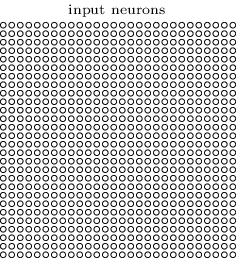
\includegraphics[width=0.25\linewidth]{neuraon}
	\caption{Ilustrasi Citra 28x28 Piksel (Nielsen., 2015)}
	\label{fig:neuraon}
\end{figure}

Seperti jaringan syaraf tiruan pada umumnya, setiap neuron dari input
terhubung dengan layer dari hidden neuron. Sedikit berbeda, pada CNN neuron 
input tidak terhubung secara \emph{fully-connected} dengan setiap hidden neuron, tetapi 
hanya region lokal kecil dari input terhubung dengan sebuah hidden neuron
(Nielsen., 2015). Pada Gambar 3.8 terlihat bahwa hanya sebagian kecil region
yang \emph{localized} dari input neuron yang terhubung dengan hidden neuron.
% TODO: \usepackage{graphicx} required
\begin{figure}[H]
	\centering
	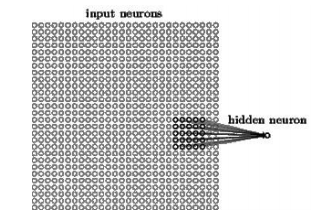
\includegraphics[width=0.5\linewidth]{hidenneuron}
	\caption{Ilustrasi \emph{local receptive fields} (Nielsen., 2015)}
	\label{fig:hidenneuron}
\end{figure}

Pada Gambar 3.9 setiap neuron pada hidden layer terhubung dengan
region berukuran 5 × 5 piksel pada neuron input. Region pada input layer inilah
yang dinamakan dengan \emph{local receptive fields} dan setiap koneksi memiliki bobot
yang akan disesuaikan seiring dengan proses pelatihan. Selain itu hidden neuron 
juga memiliki dan mempelajari bias secara keseluruhan. Oleh karena itu, setiap
hidden neuron dilatih untuk menganalisa masing-masing local receptive fields yang 
bersesuaian.

Tahap selanjutnya, local receptive fields akan digeser (slide) sepanjang 
ukuran citra dari posisi paling kiri atas hingga kanan bawah. Setiap local receptive
fields akan memiliki pasangan hidden neuron yang berbeda pada hidden layer.
Ilustrasi proses pergeseran \emph{local receptive fields} terdapat pada Gambar 3.9 dan
Gambar 3.10 berikut.
% TODO: \usepackage{graphicx} required
\begin{figure}[h]
	\centering
	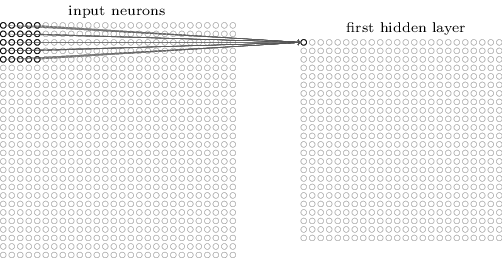
\includegraphics[width=0.65\linewidth]{neuron2}
	\caption{Ilustrasi Pergesaran \emph{local receptive fields} (Nielsen., 2015)}
	\label{fig:neuron2}
\end{figure}

Selanjutnya \emph{local receptive fields} akan digeser sebanyak satu piksel ke
kanan seperti pada Gambar 3.8 dan terhubung dengan hidden neuron yang 
berbeda dengan local receptive fields sebelumnya.
% TODO: \usepackage{graphicx} required
\begin{figure}[h]
	\centering
	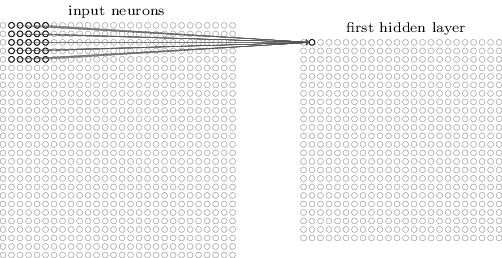
\includegraphics[width=0.65\linewidth]{neuron3}
	\caption{Ilustrasi Pergeseran dengan Stride = 1 (Nielsen., 2015)}
	\label{fig:neuron3}
\end{figure}

Pergeseran piksel dengan stride = 1 di ilustrasikan pada Gambar 3.9.Proses ini berlangsung hingga \emph{local receptive fields} berada pada posisi 
piksel paling kanan bawah. Sehingga setelah proses slide dilakukan akan terbentuk
hidden layer dengan ukuran sesuai dengan ukuran local receptive fields dan 
panjang pergeseran (stride) yang digunakan (Nielsen, 2015). Maka jika citra dengan ukuran 28 × 28 piksel dan digunakan \emph{local receptive fields}
dengan ukuran 5 × 5, dan digeser dengan stride = 1, maka akan terbentuk
hidden layer dengan ukuran 24 × 24 neuron.
%================================================ Shared Weight
\subsection{Shared Weight}
Pada CNN, sebuah neuron pada hidden layer yang terhubung dengan 5 × 5 
neuron pada input layer (sesuai dengan ukuran \emph{local receptive fields} yang 
digunakan). Hal ini menunjukkan bahwa neuron tersebut memiliki sebuah bias dan 
matriks bobot dengan ukuran 5 × 5 yang menghubungkan 5 × 5 neuron inputnya.
Matriks bobot ini, dalam CNN, disebut sebagai kernel. Matriks bobot pada jaringan 
syaraf tiruan biasa sedikit berbeda dengan matriks bobot pada CNN, yaitu nilai 
matriks bobot pada CNN bernilai sama untuk setiap 24 × 24 neuron pada hidden 
layer. Hal tersebut menunjukkan bahwa semua neuron pada hidden layer akan 
mendeteksi fitur yang sama dengan lokasi pada input citra yang berbeda (Nielsen., 
2015).

%!=============================================== Konvolusi
\subsection{Konvolusi}
Lapisan yang pertama kali akan dilewati oleh data masukan adalah lapisan konvolusi, bertujuan untuk memperoleh feature map yang merepresentasikan masukan. Parameter yang digunakan untuk menentukan ukuran feature map keluaran berupa filter, ukuran dari filter, besarnya langkah pergeseran filter pada operasi konvolusi atau biasa disebut stride, dan ukuran padding. Cara menghitung ukuran dari keluaran operasi konvolusi ditunjukkan pada Persamaan 3.26 dan 3.27  berikut(Nielsen., 2015):
\begin{equation}
H_0 = \frac{H-F+2P}{S}+1
\end{equation}

\begin{equation}
W_0 = \frac{W_i-F+2P}{S}+1
\end{equation}
Keterangan : \\
\(H_0\) = tinggi fitur map keluaran
\\
\(W_0\) = lebar fitur map keluaran\\
\(H_i\) = tinggi fitur map masukan
\\
\(W_i\) = lebar fitur map masukan
\\
\(F\)  = ukuran filter
\\
\(P\)  = ukuran padding
\\
\(S\)  = ukuran stride 

Nilai semua elemen pada persamaan tersebut harus merupakan bilangan bulat karena akan merepresentasikan suatu ukuran feature map. Apabila terdapat salah satu nilai yang bukan merupakan bilangan bulat, nilai tersebut harus dibulatkan dengan melakukan pembulatan kebawah. Adapun cara menghitung nilai keluaran dari proses konvolusi dapat dilihat pada Persamaan 3.278berikut(Nielsen., 2015):
\begin{equation}
O_{mn}=\sum I^k_{i,j} . F_{i,j}
\end{equation}
Keterangan :
\\
\(O_{mn}\)= elemen matriks keluaran pada baris ke-m kolom ke –n.
\\
\(I^k_{i,j}\)= elemen matriks masukan bagian ke-k pada baris ke-i kolom ke-j. 
\\
\(F_{i,j}\)= elemen matriks filter pada baris ke-i kolom ke –j.
%!=============================================== Fungsi Aktivasi
\subsection{Fungsi Aktivasi}
Salah satu faktor signifikan mempengaruhi kinerja algoritme Convolutional Neural Network adalah penerapan fungsi aktivasi dalam jaringan. Fungsi ini membantu menyelesaikan permasalah-permasalahan yang bersifat non-trivial dalam suatu jaringan dengan cara mengambil sebuah nilai dan melakukan operasi matematika. Fungsi aktivasi ini diletakkan di perhitungan akhir dari keluaran feature map atau setelah layer konvolusi dan subsampling layer. Fungsi aktivasi yang sering digunakan adalah Rectified Linear Unit (ReLU) karena fungsi ini lebih cepat daripada fungsi aktivasi non-linear lainnya seperti sigmoid atau tanh. Fungsi ReLU dapat dilihat pada Persamaan 3.29 dan 3.30(Nielsen., 2015):
\begin{equation}
f(x) = ReLU(x) =max(0,x)
\end{equation}
\begin{equation}
	f(x)= 0 \ jika \ x \leq{0} \ atau \ x \ jika > 0
\end{equation}
\section{Evaluasi}
\subsection{Confussion Matrix}
Pengukuran evaluasi dari pengujian dapat dilakukan menggunakan \emph{confusion matrix}. tabel \emph{confusion matrix} merupakan tabel klasifikasi yang bersifat prediktif seperti ditunjukan pada Gambar 3.11. Evaluasi menggunakan confussion matrix dapat digunakan untuk mengukur nilai akurasi dengan Persaman 3.31.
% TODO: \usepackage{graphicx} required
\begin{figure}[H]
\centering
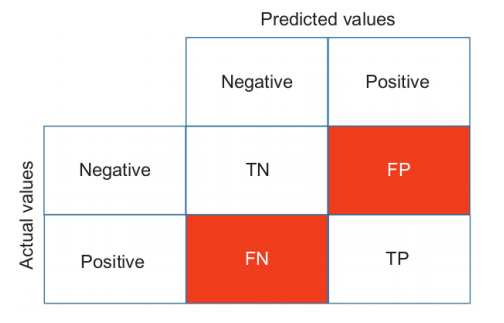
\includegraphics[width=0.7\linewidth]{confusion}
\caption{Confusion Matrix (Leonard., 2017)}
\label{fig:confusion}
\end{figure}
\begin{equation}
akurasi = \frac{TP}{TP+FP}
\end{equation}
Dengan :\\
$TP$ = True Positif, objek berupa gestur tangan dan terkenali\\
$FP$ = False Positif, objek berupa gestur tangan tapi tidak terkenali
\subsection{Average Precicion(AP)}
\emph{Average Precicion} adalah metrik populer untuk melakukan evaluasi pada objek detektor seperti \emph{Faster-RCNN, SSD, dan lainnya}. AP menghitung nilai rata rata nilai presisi untuk nilai recall 0 hingga 1 (Hui., 2018). Evaluasi deteksi menggunakan konsep IoU(\emph{intersection over union})
IoU menghitung interseksi kedua bounding boxes dimana terdiri dari ground truth dan prediksi dari bounding box digambarkan pada Gambar 3.12 dan perhitungan IoU pada Persamaan 3.32.
% TODO: \usepackage{graphicx} required
\begin{figure}[H]
	\centering
	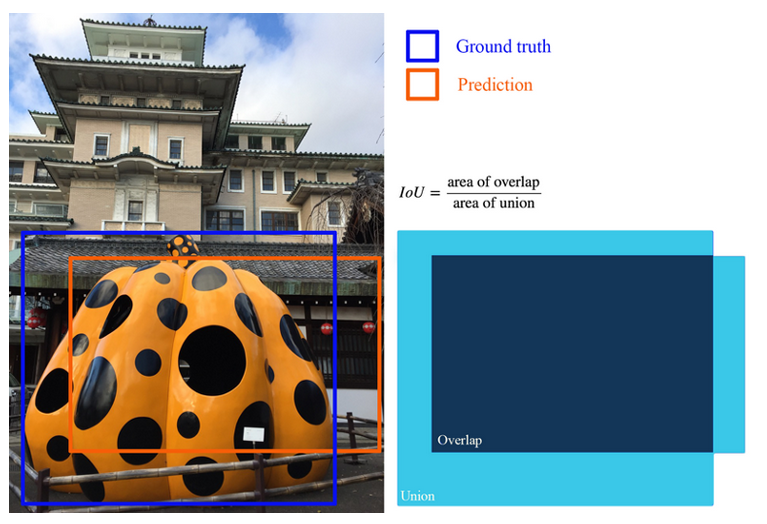
\includegraphics[width=0.7\linewidth]{iou}
	\caption{Ilustrasi IoU(Hui., 2018)}
	\label{fig:iou}
\end{figure}
\begin{equation}
	IoU=\frac{area\_of\_overlap}{area\_of\_union}
\end{equation}

IoU yang digunakan untuk memprediksi suatu bounding box, apabila nilai IoU melebihi \emph{threshold} yang ditentukan maka akan terdeteksi sebuah objek.
Sebaliknya jika IoU kurang dari batas yang ditentukan maka menandakan tidak terdeteksi apapun pada citra. 

Terdapat 4 kategori dalam penentuan deteksi yaitu,
FN(\emph{False Negative}) terdapat objek namun tidak mendeteksi apapun.
FP(\emph{False Positive}) tidak terdapat objek namun hasilnya terdeteksi.
TP(\emph{True Positive}) terdapat objek dan terdeteksi.
TN(\emph{True Negative}) akan terjadi jika tidak ada objek dan tidak terdeteksi apapun.
Berdasarkan nilai yang didapat maka diketahui presisi dan recall menggunakan Persamaan 3.33 dan Persamaan 3.34 (Hui., 2018).
\begin{equation}
	presisi = \frac{TP}{TP+FP}
\end{equation}
\begin{equation}
recall = \frac{TP}{TP+FN}
\end{equation}
Metrik untuk mengukur detektor dari \emph{object detection} menggunakan mAP \emph{(mean average precicion)}. Nilai mAP dan AP dalam COCO dataset tidak memiliki perbedaan, dimana mAP adalah rata rata dari setiap AP yang memiliki nilai IoU sebagai \emph{threshold}. Total metrik evaluasi pada COCO memiliki 12 metrik seperti pada Gambar 3.13 (Chen et al., 2015).
% TODO: \usepackage{graphicx} required
\begin{figure}[H]
	\centering
	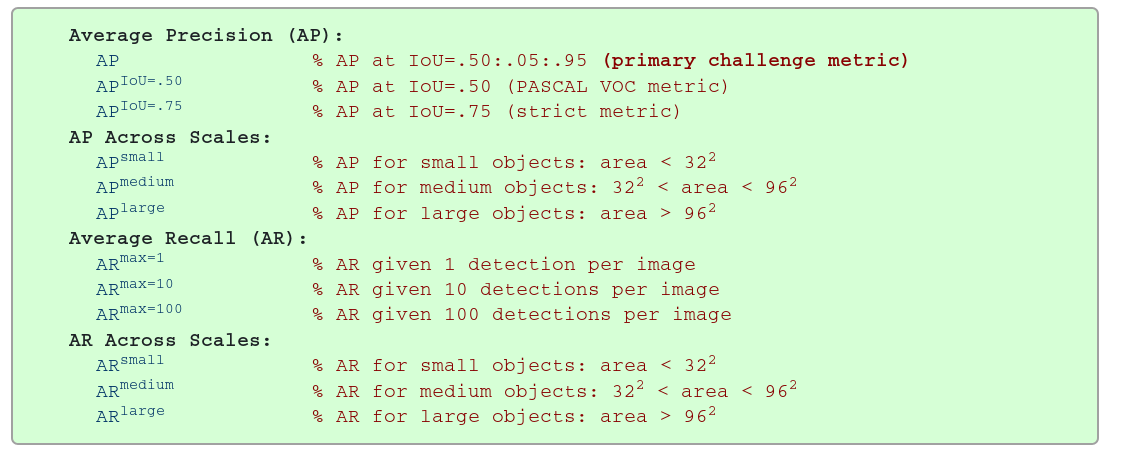
\includegraphics[width=1\linewidth]{mtrik}
	\caption{Metrik Evaluasi COCO (Chen et al., 2015)}
	\label{fig:mtrik}
\end{figure}


\chapter{METODOLOGI PENELITIAN}
\section{Studi Literatur}
Studi literature dilakukan dengan mempelajari penelitian yang berkaitan dengan materi \emph{hand gesture recognition}, \emph{Retinex} dan \emph{Convolutional Neural Network} yang  diperoleh dari berbagai sumber seperti buku, artikel, jurnal dan sumber lain yang diperoleh dari internet.
\section{Alat dan Bahan}
\subsection{Alat}
Penelitian ini menggunakan beberapa peralatan yang digunakan untuk membantu kegiatandari mulai pengumpulan data hingga pengujian sistem, beberapa peralatan tersebut adalah sebagai berikut :
\begin{enumerate}
\item PC/Laptop dengan spesifikasi processor Intel (R) Core i5-8300H CPU @2,4 GHz, GPU NVIDIA 1050, RAM 8 GB, sistem operasi Linux 64 bit.
\item Webcam Logitech C270
\item Dimmer
\item Kain	
\item Lux Meter
\end{enumerate}
Laptop merupakan peralatan yang paling utama yang digunakan untuk melakukan proses pengolahan citra dengan webcam sebagai alat untuk menangkap citra. Lux meter digunakan untuk mengukur intensitas cahaya saat pengambilan data dan pengujian data dengan menurunkan intensitas cahaya yang diatur menggunakan dimmer. Penggunaan kain bersifat opsional untuk latar belakang yang bervariasi.
\subsection{Bahan}
Bahan yang digunakan untuk melakukan penelitian ini berupa dataset, diantaranya sebagai berikut:
\begin{enumerate}
	\item Dataset gestur tangan ASL 
	\item Dataset gambar tangan
\end{enumerate}
Dataset gestur tangan ASL merupakan dataset dari \emph{Massey University} yang digunakan untuk melatih model pengenalan gestur tangan, sementara dataset gambar tangan merupakan dataset untuk melakukan pelatihan deteksi tangan. Dataset gambar tangan diambil dari 3 subjek yang diambil gambar menggunakan webcam.
\section{Prosedur Kerja}
\subsection{Analisis dan Perancangan Sistem}
Alur penelitian yang akan dilakukan dalam penelitian ini memiliki beberapa tahapan diantaranya pengambilan dataset gestur, training data dan tahap paling akhir adalah pengujian. Alur kegiatan penelitian yang akan dilakukan secara garis besar ditunjukan pada Gambar 4.1.
% TODO: \usepackage{graphicx} required
\begin{figure}[H]
	\centering
	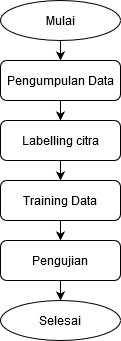
\includegraphics[width=0.2\linewidth]{Rencana}
	\caption{Alur Kegiatan Penelitian}
	\label{fig:screenshot006}
\end{figure}
Rancangan pengujian sistem ditunjukan pada Gambar 4.2 yang dimulai dengan \emph{input} dari webcam secara \emph{realtime}, sehingga setiap frame akan di proses pada tahap berikutnya.
Setiap frame dengan citra RGB akan dilewatkan pada algoritme \emph{Retinex} untuk dilakukan perbaikan kualitas citra dengan harapan meningkatkan kontras pada sebuah citra.
% TODO: \usepackage{graphicx} required
\begin{figure}[H]
	\centering
	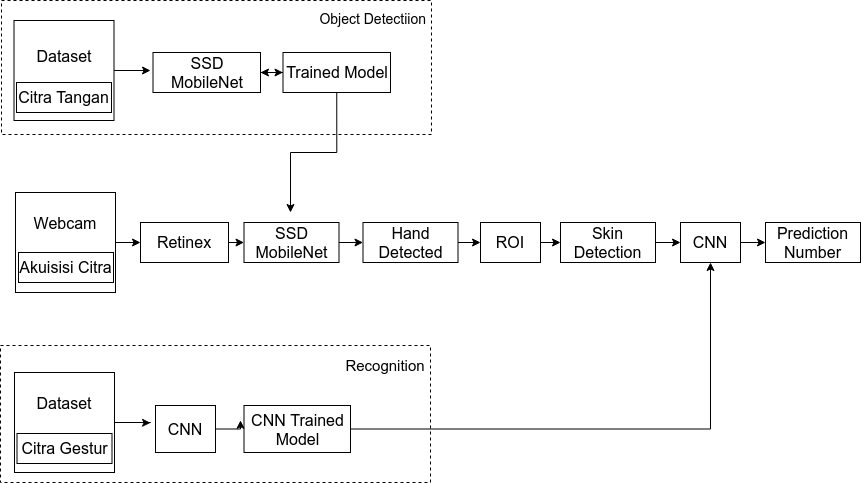
\includegraphics[width=1.1\linewidth]{rancanganedit}
	\caption{Rancangan Sistem}
	\label{fig:rancangan}
\end{figure}
\noindent Citra yang mengalami peningkatan kontras kemudian sistem akan melakukan deteksi tangan dengan \emph{SSD MobileNet} yang kemudian citra tangan tersebut akan diambil sebagai ROI. 
Citra hasil ROI akan dilakukan segmentasi menggunakan \emph{skin detection}. Hasil segmentasi akan diklasifikasikan dengan model CNN yang telah di training sebelumnya.
Keluaran dari sistem ini akan menampilkan klasifikasi angka yang terdeteksi.

Penelitian yang digambarkan pada rencana sistem memiliki 3 bagian penting diantaranya \emph{Retinex}, \emph{SSD MobileNet} dan \emph{Convolutional Neural Network}.
Peranan Retinex pada penelitian ini merupakan solusi untuk mengatasi permasalahan intensitas cahaya, sehingga pada dataset yang dilatih tidak perlu menggunakan variasi intensitas yang rendah. Penggunaan SSD dengan arsitektur \emph{MobileNet} bertujuan untuk mempercepat waktu komputasi supaya tidak terlalu berat dengan harapan lebih cepat. \emph{Convolutional Neural Network} sendiri digunakan untuk melakukan ekstraksi fitur dari sebuah citra. Ekstraksi fitur ini sangat sering digunakan dalam pemrosesan sebuah citra untuk memperoleh informasi. 
\subsection{Pra-proses}
Tahap pra-proses pada penelitian ini terdapat pada proses \emph{enhancement} yang dilakukan oleh \emph{Retinex}. Citra dengan intensitas cahaya rendah akan dilakukan proses perbaikan dahulu sebelum dilakukan proses deteksi maupun pengenalan. \emph{Input} citra untuk proses \emph{Retinex} menggunakan 3 kanal(R,G,B).

Proses pertama yang dilakukan adalah membuat filter \emph{gaussian} menggunakan Persamaan 3.14 dengan permisalan $\sigma$ = 10.

\noindent
$\left[
\begin{matrix}
	\frac{1}{2\pi(10)^2}\times \exp^{-\frac{(-1)^2+1^2}{2(10)^2}} & \frac{1}{2\pi(10)^2}\times \exp^{-\frac{0^2+1^2}{2(10)^2}} &\frac{1}{2\pi(10)^2}\times \exp^{-\frac{1^2+1^2}{2(10)^2}} \\
	\frac{1}{2\pi(10)^2}\times \exp^{-\frac{(-1)^2+0^2}{2(10)^2}} & \frac{1}{2\pi(10)^2}\times \exp^{-\frac{0^2+0^2}{2(10)^2}} &\frac{1}{2\pi(10)^2}\times \exp^{-\frac{1^2+0^2}{2(10)^2}} \\
	\frac{1}{2\pi(10)^2}\times \exp^{-\frac{(-1)^2+(-1)^2}{2(10)^2}} & \frac{1}{2\pi(10)^2}\times \exp^{-\frac{0^2+(-1)^2}{2(10)^2}} &\frac{1}{2\pi(10)^2}\times \exp^{-\frac{1^2+(-1)^2}{2(10)^2}} 	
\end{matrix}
\right]$

\noindent Filter \emph{gaussian} yang dihasilkan menggunakan $\sigma$=10 adalah sebagai berikut.

\noindent
$\left[
\begin{matrix}
	0,001575 & 0,001583 & 0,001575
	 \\
	0,001583 & 0,001591 & 0,001583
	\\
	0,001575 & 0,001583 & 0,001575
\end{matrix}
\right]$

\noindent Berdasarkan Persamaan 3.15, integral dari filter \emph{gaussian} harus sama dengan 1. Integral dari filter tersebut dapat dicari dengan menjumlahkan semua elemen. Pada kasus ini nilai integral atau jumlahan dari elemen adalah 0.0142288. Apabila hasil dari integral tersebut tidak sama dengan 1 maka akan dikalikan menggunakan formula berikut.\\
$
new\_a_{(x,y)}=a_{(x,y)}\times\frac{1}{total}
$\\
$
new\_a_{(-1,1)}=0,001575\times\frac{1}{0,142288}=0,110740\\
new\_a_{(-1,0)}=0,001583\times\frac{1}{0,142288}=0,111295
$

\noindent Perhitungan nilai filter \emph{gaussian} dilakukan untuk setiap distribusi kernel sehingga membentuk filter dengan nilai baru. Nilai filter yang baru menghasilkan hasil integral sama dengan 1.\\

\noindent
$\left[
\begin{matrix}
0,110740&0,111295&0,110740\\
0,111295&0,111853&0,111295\\
0,110740&0,111295&0,110740
\end{matrix}
\right]$

\noindent Filter \emph{gaussian} ini akan dikonvolusikan dengan input citra, contoh citra yang akan dikonvolusikan sebagai berikut.

\noindent
$I_{(x,y)}=\left[
\begin{matrix}
0&0&0&0&0&0\\
0&120&	125&	124&	126&0\\
0&126&	135&	146&	189&0\\
0&170&	187&	200&	210&0\\
0&189&	188&	197&	221&0\\
0&0&0&0&0&0
\end{matrix}
\right]$*
$F_{(x,y)}=\left[
\begin{matrix}
0,110740 &0,111295&0,110740\\
0,111295&0,111853&0,111295\\
0,110740&0,111295&0,110740\\
\end{matrix}
\right]$

\noindent Perhitungan konvolusi untuk mendapatkan dimensi yang sama dengan citra \emph{input} digunakan \emph{zero padding}. Hasil konvolusi di ilustrasikan pada perhitungan berikut.

\noindent $O_{(1,1)}=$(0*0,110740)+(0*0.111295)+(0*0,110740)+(0*0,111295)+(120*0,111853)\\
+(125*0,111295)+(0*0,110740)+(126*0,111295)+(135*0,110740)=56,307698

\noindent$O_{(2,1)}=$(0*0,110740)+(0*0,111295)+(0*0,110740)+(120*0,111295)+(125*0,111853)\\
+(124*0,111295)+(126*0,110740)+(135*0,111295)+(146*0,110740)=86,284315

\noindent Konvolusi dilakukan dengan pergeseran 1 piksel sehingga menghasilkan citra dengan dimensi yang sama. Hasil konvolusi($O_{(x,y)}$) merupakan nilai dari Persamaan 3.13 yang mendapatan nilai sebagai berikut.

\noindent
$O_{(x,y)}=\left[
\begin{matrix}
56,307698&	86,284315&	93,934305&	65,097310\\
95,945406&	148,09183&	160,21034&	110,66494\\
110,65489&	170,91206&	185,90262&	129,36380\\
81,692776&	125,77508&	133,77841&	92,165220
\end{matrix}
\right]$\\
$\log O_{(x,y)}=\left[
\begin{matrix}
1,750568&	1,935932&	1,972825&	1,813563\\
1,982024&	2,170531&	2,204691&	2,044011\\
2,043971&	2,232773&	2,269286&	2,111813\\
1,912183&	2,099594&	2,126386&	1,964568

\end{matrix}
\right]$

\noindent Nilai akhir dari \emph{Single Scale Retinex} adalah pengurangan antara hasil logaritmik citra asli dengan logaritmik citra hasil konvolusi dimana dituliskan dalam Persamaan 3.17. Berikut adalah hasil \emph{Single Scale Retinex}($\sigma$=10).

\noindent
$R_{(SSR(\sigma=10))=}\left[
\begin{matrix}
0,328612&	0,160977&	0,120596&	0,286806\\
0,118345&	-0,040198&	-0,04033&	0,232450\\
0,186477&	0,039068&	0,031743&	0,210405\\
0,364278&	0,174563&	0,168079&	0,379824
\end{matrix}
\right]$

\noindent Perhitungan \emph{Multiscale Retinex} jumlahan dari setiap \emph{Single Scale Retinex}. \emph{Single Scale Retinex} dengan $\sigma$=65 dan $\sigma$=180 didapatkan nilai sebagai berikut.

\noindent
$R_{(SSR(\sigma=65))=}\left[
\begin{matrix}
0,329257&	0,161283&	0,120802&	0,287442\\
0,118596&	-0,040252&	-0,040368&	0,232871\\
0,186859&	0,039126&	0,031776&	0,210871\\
0,364991&	0,174929&	0,168434&	0,380586
\end{matrix}
\right]$

\noindent
$R_{(SSR(\sigma=180))=}\left[
\begin{matrix}
0,329271&	0,161289&	0,120806&	0,287455\\
0,118601&	-0,040253&	-0,040369&	0,232879\\
0,186867&	0,0391275&	0,0317764&	0,210880\\
0,365006&	0,1749365&	0,1684419&	0,380602
\end{matrix}
\right]$

\noindent \emph{Multiscale Retinex} memiliki bobot pada setiap skala, dimana jika bobot dijumlahkan = 1. Bobot tersebut dikalikan dengan citra untuk masing masing skala, sehingga mendapatkan nilai berikut dengan masing masing bobot$\omega_n=0.3, 0.3, 0.4$.

\noindent
$R_{(SSR(\sigma=10))*0,3}\left[
\begin{matrix}
0,098583&	0,048293&	0,036178&	0,086041\\
0,035503&	-0,012059&	-0,012101&	0,069735\\
0,055943&	0,011720&	0,009523&	0,063121\\
0,109283&	0,052368&	0,050423&	0,113947
\end{matrix}
\right]$

\noindent
$R_{(SSR(\sigma=65))*0,3}\left[
\begin{matrix}
0,098777&	0,048385&	0.036240&	0.086232\\
0,035578&	-0,012075&	-0.012110&	0.069861\\
0,056057&	0,011737&	0.009532&	0.063261\\
0,109497&	0,052478&	0.050530&	0.114175
\end{matrix}
\right]$

\noindent
$R_{(SSR(\sigma=180))*0,4}\left[
\begin{matrix}
0,131708&	0,064515&	0,048322&	0,114982\\
0,047440&	-0,016101&	-0,016147&	0,093151\\
0,074746&	0,015651&	0,012710&	0,084352\\
0,146002&	0,069974&	0,067376&	0,152240
\end{matrix}
\right]$

\noindent Setiap nilai \emph{Single Scale Retinex} dijumlahkan seperti pada Persamaan 3.18, kemudian hasil dari penjumlahan akan dilakukan normalisasi dengan hasil akhir yang dibulatkan.

\noindent
$R_{(MSR)}=\left[
\begin{matrix}
0,329069&	0,161194&	0,120742&	0,287256\\
0,118523&	-0,040236&	-0,040360&	0,232748\\
0,186748&	0,039109&	0,031766&	0,210735\\
0,364783&	0,174822&	0,168331&	0,380363
\end{matrix}
\right]$

\noindent Normalisasi = $\frac{(ABS(Nilai_{(x,y)})-Nilai\_min)}{(Nilai\_max-Nilai\_min)}$$\times$255

\noindent
$R_{(MSR)}=\left[
\begin{matrix}
224&	122&	98&		198\\
96&		0&		1&		165\\
138&	48&		44&		152\\
246&	130&	126&	255

\end{matrix}
\right]$\\
Gambar 4.3 menunjukan ilustrasi peningkatan kualitas citra dengan intensitas cahaya rendah dikenai algoritme \emph{retinex} sehingga menghassilkan citra dengan pengingkatan kontras.
% TODO: \usepackage{graphicx} required
\begin{figure}[H]
	\centering
	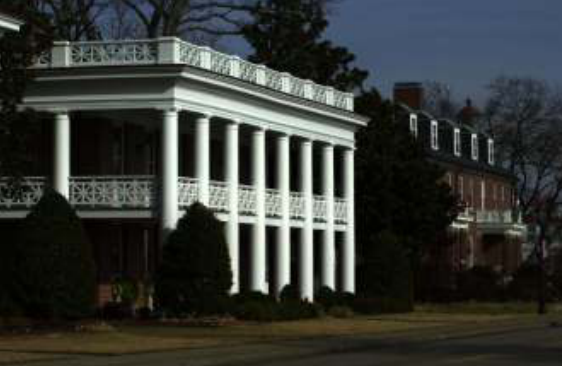
\includegraphics[width=0.4\linewidth]{ret1}
	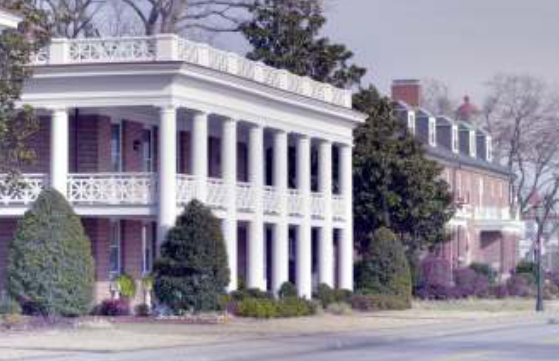
\includegraphics[width=0.4\linewidth]{ret2}\\
	a \ \ \ \ \ \ \ \ \ \ \ \ \ \ \ \ \ \ \ \  \ \ \ \ \ \ \ \ \ \ \ \ \ \ \ \ \ \ \ \ \ \ \ \ \ \ \ \ \ \ \ \ b
	\caption{Ilustrasi Perbaikan Kontras Menggunakan Retinex (a) Citra Asli; (b) Citra Hasil Perbaikan(Petro et al., 2014)}
	\label{fig:ret1}
	\label{fig:ret2}
\end{figure}


\subsection{Pengumpulan Data}
Data pelatihan dibagi menjadi dua, yaitu dataset citra gestur tangan yang mengacu pada ASL dan dataset citra tangan biasa untuk \emph{object detection}.
Kedua dataset ini merupakan dua hal yang berbeda tujuan. 
Dataset ASL digunakan untuk model pengenalan gestur ASL dan dataset citra tangan digunakan untuk model deteksi tangan.

Dataset gestur tangan ASL menggunakan dataset public dari \emph{Massey University}. Dataset tersebut berisi 2425 citra yang dibagai dalam 36 kelas, yaitu 26 untuk huruf A-Z dan 10 kelas untuk angka 0-9. Pengambilan dataset dilakukan oleh 5 individu dengan variasi cahaya yang berbeda(Barczak et al., 2011).
Acuan dalam penelitian ini menggunakan dataset angka 0 sampai 9, dengan citra yang sudah di segmentasi.
Dataset ini akan dilatih dalam CNN untuk pengenalan gestur tangan.
Pengambilan dataset \emph{Massey University} dilakukan menggunakan \emph{green screen} sehingga mudah untuk disegmentasi, setup pengambilan dataset dilakukan dengan skema seperti Gambar 4.4 (Barczak et al., 2011).

Pengambilan dataset berikutnya berbeda dengan dataset ASL, dataset berikutnya diambil menggunakan webcam untuk keperluan deteksi tangan, citra diambil dari 10 orang dengan random pose. Dataset ini digunakan untuk pelatihan pada \emph{object detection}. 
Pengambilan dataset dilakukan masing masing 100 capture untuk setiap orang, sehingga pada dataset ini diperoleh 1000 citra. 

Proses pengumpulan dataset tidak menghiraukan nilai intensitas cahaya karena permasalahan pencahayaan sudah diatasi pada algoritme \emph{Retinex}, namun akan tetap diukur kondisi intensitas pada lingkungan tersebut menggunakan lux meter. Penggunaan dataset ASL dari \emph{Massey University} tidak memiliki keterangan nilai intesitas cahaya, namun berdasarkan citra tersebut cenderung memiliki nilai intensitas yang tinggi, dimana dapat dilihat pada isi dataset. Tujuan dari dataset yang dilatih hanya untuk membuat model klasifikasi dan deteksi tanpa memperhitungkan intensitas cahaya rendah.
% TODO: \usepackage{graphicx} required
\begin{figure}[H]
	\centering
	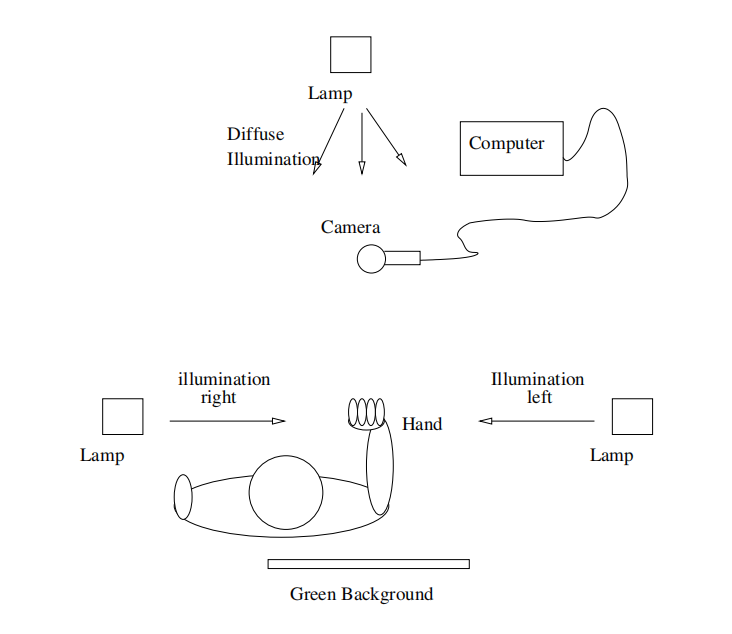
\includegraphics[width=0.8\linewidth]{setup}
	\caption{Skema Pengambilan Dataset (Barczak et al., 2011)}
	\label{fig:setup}
\end{figure}
\section{Proses Pelatihan}
Proses pelatihan dalam penelitian ini dibagi menjadi dua bagian, yaitu pelatihan object detection dan pelatihan gestur recognition.
\subsection{Pelatihan Gesture Recognition}
Dataset pada pelatihan \emph{gesture recognition} menggunakan dataset dari \emph{Massey Univertisy} yang di labeli sesuai acuan ASL dari angka 0 hingga 9. Jumlah dataset adalah 700 citra kemudian dibagi yang akan dibagi dalam \emph{train} dan \emph{test} menggunakan \emph{k-fold cross validation} dengan k = 5.
Proses pelatihan untuk pengenalan gestur tangan menggunakan teknik \emph{transfer learning} yang memiliki kelebihan pada waktu pelatihan dan penggunaan dataset yang cenderung sedikit. \emph{Pre-trained} model yang digunakan adalah \emph{MobileNetV2}. \emph{Pre-trained} model memiliki pengetahuan dari dataset yang telah dilatih sebelumnya, pada \emph{MobileNetV2} telah dilatih menggunakan dataset dari \emph{ImageNet}, kemudian pengetahuan tersebut akan di pindahkan ke model baru dan dilatih sesuai dataset baru, sehingga memiliki keluaran dalam bentuk klasifikasi atau tugas sesuai yang diinginkan.

Masukan citra memiliki dimensi 224x224 piksel yang terdiri 3 channel RGB, sehingga node \emph{input} berjumlah 50176 dengan range 0-255 untuk setiap piksel. Arsitektur jaringan pada pelatihan ini dilakukan dengan mengganti bagian blok klasifikasi dari \emph{MobileNetV2} menjadi klasifikasi dataset ASL. 
Arsitektur transfer learning dapat dilihat pada Gambar 4.5.
% TODO: \usepackage{graphicx} required
\begin{figure}[H]
	\centering
	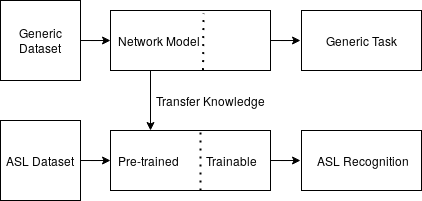
\includegraphics[width=0.8\linewidth]{transfer}
	\caption{Transfer Learning Pelatihan Gestur}
	\label{fig:asritrkturku}
\end{figure}

\subsection{Pelatihan Object Detection}
Proses pelatihan pada \emph{object detection} menggunakan \emph{pre-trained model SSD MobilenetV2 COCO} yang sudah di latih sebelumnya dengan dataset COCO.
Dataset yang baru akan dilatih menggunakan \emph{pre-trained} model, sehingga dengan pengetahuan yang sudah ada dilatih agar menghasilkan model baru sesuai dengan \emph{output} yang diinginkan. 
Dataset yang akan dilatih sejumlah 1000 citra yang telah dilabeli secara manual dengan pembagian 80\% \emph{training} dan 20\% \emph{testing}.
Arsitektur yang digunakan dalam pelatihan \emph{object detection} dapat dilihat pada Gambar 4.6.
\begin{figure}[H]
	\centering
	\includegraphics[width=0.7\linewidth]{"v2"}
	\caption{Arsitektur Mobilenet V2 (Sandler et al., 2018)}
	\label{fig:v2}
\end{figure}
%----------------------------------PENGUJIAN-------------------------------------
\section{Pengujian dan Evaluasi}
Pengujian dan evaluasi adalah tahap untuk mengukur performa dari sebuah sistem. Pengujian ini akan dibagi menjadi 6 tahap, yaitu evaluasi deteksi tangan, evaluasi pengenalan gestur, pengujian deteksi tangan menggunakan \emph{Retinex}, pengujian pengenalan gestur tangan menggunakan \emph{Retinex}, pengujian SNR dan pengujian keseluruhan sistem. 
Setiap pengujian yang menggunakan Retinex dilakukan hal yang sama, yaitu dengan menurunkan intensitas cahaya.
%------------------------------------PENGUJIAN DETEKSI------------------------
\subsection{Evaluasi Deteksi Tangan}
Evaluasi model deteksi tangan dilakukan setelah \emph{training} menggunakan metrik \emph{mean average precicion} (mAP). \emph{Mean average precicion} merupakan metrik yang populer untuk mengevaluasi model dari detektor. \emph{Mean average precicion} merupakan rata rata dari \emph{Average Precicion} (AP) pada setiap nilai IoU. Sesuai dengan acuan COCO dataset untuk mengevaluasi model pada \emph{object detection} dengan menghitung mAP dari IoU=0,5 hingga 0,95 dengan pertambahan 0,05.
\subsection{Evaluasi Pengenalan Gestur Tangan}
Evaluasi model CNN untuk pengenalan gestur tangan didapatkan saat \emph{training} dan \emph{testing} menggunakan \emph{k-fold cross validation} dengan k = 5, dimana dilakukan validasi sebanyak 5 kali dengan skenario pengujian yang berbeda pada proses \emph{training} dan \emph{testing}.
\emph{Training accuracy} dan \emph{testing accuracy} didapatkan pada setiap \emph{fold}. Model dengan akurasi terdinggi akan digunakan sebagai model untuk pengenalan gestur tangan.
\subsection{Pengujian SNR}
SNR\emph{(Signal to Noise Ratio)} adalah ukuran untuk mengukur kualitas citra terhadap citra yang dilakukan perbaikan. Citra hasil perbaikan dibandingkan dengan citra asli untuk mendapatkan nilai SNR nya. Nilai SNR yang tinggi mengindikasikan kualitas citra yang semakin baik karena rasio sinyal terhadap metode juga tinggi, sebaliknya nilai SNR yang rendah berarti kualitas citra yang di hasilkan semakin buruk atau semakin kecil dalam peningkatan kualitas citra. Pengujian SNR ini dilakukan untuk menentukan nilai dari parameter \emph{retinex} yang akan dipakai pada sistem.
\subsection{Pengujian Deteksi Tangan Menggunakan Retinex}
Tujuan pengujian deteksi tangan dilakukan untuk menguji sistem dalam melakukan deteksi tangan terkait dengan penurunan intensitas cahaya. Ilustrasi pengujian deteksi tangan digambarkan pada Gambar 4.7. Pengujian dilakukan dengan kondisi cahaya awal sesuai yang terjadi pada ruangan. Pada kondisi awal tersebut akan dilakukan deteksi tangan, setiap hasil dari deteksi tersebut berupa \emph{true positive} atau \emph{false positive}. Hasil deteksi akan dicatat dalam bentuk tabel seperti pada Tabel 4.1.
% TODO: \usepackage{graphicx} required
\begin{figure}[H]
	\centering
	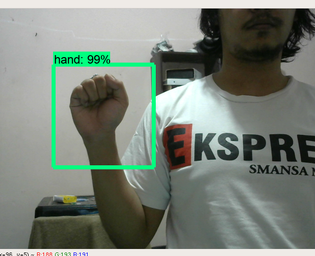
\includegraphics[width=0.72\linewidth]{deteksihand}
	\caption{Ilustrasi Pengujian Deteksi Tangan}
	\label{fig:deteksihand}
\end{figure}
% TODO: \usepackage{graphicx} required
\begin{figure}[H]
	\centering
	\includegraphics[width=0.4\linewidth]{"skema pengujian deteksi tangan"}
	\caption{Skema Kegiatan Pengujian Deteksi Tangan}
	\label{fig:skema-objek-deteksi}
\end{figure}
Pada pengujian ini alur kegiatan yang dilakukan saat pengujian deteksi tangan dapat dilihat pada Gambar 4.8. Pengujian deteksi tangan dilakukan secara manual oleh 3 subjek yang berbeda, setiap subjek akan dicatat apakah sistem mampu mendeteksi tangan atau tidak pada intensitas cahaya pada saat itu selama 10 kali, kemudian dilakukan penurunan intensitas sebesar 50\% untuk kondisi selanjutnya dan dilakukan hal yang sama. Penurunan ini dilakukan hingga nilai lux yang terukur bernilai kurang dari atau sama dengan 50lux. Evaluasi pengujian dilakukan dengan \emph{confussion matrix} menggunakan data yang dicatat pada Tabel 4.1, sehingga dapat diperoleh nilai akurasi untuk setiap kondisi lux dari hasil pengujian.
\begin{table}[H]
	\caption{Pengujian Deteksi Tangan}
	\vspace{0cm}
	\centering
	\begin{tabular}{|c|c|c|c|c|c|c|c|c|c|c|c|c|c|c|c|c|c|c|c|c|c|c|c|c|c|c|c|c|c|c|}
		\hline
		Nilai Lux(X) & \multicolumn{10}{|c|}{Hasil Deteksi Subjek\_1} & \multicolumn{10}{|c|}{Hasil Deteksi Subjek\_2}& \multicolumn{10}{|c|}{Hasil Deteksi Subjek\_3}\\
		\hline X & & & &&&&&&&&&&&&&&&&&&&&&&&&&&&\\
		\hline X=X*50\% & & & &&&&&&&&&&&&&&&&&&&&&&&&&&&\\
		\hline X=X*50\% & & & & && &&&&&&&&&&&&&&&&&&&&&&&&\\
		\hline X=X*50\% & & & &&&&&&& &&&&&&&&&&&&&&&&&&&&\\
		\hline $\dots$ & & & & & &&&&&&&&&&&&&&&&&&&&&&&&&\\
		\hline X=X $\le$ 50Lux & & & &&&&&&& &&&&&&&&&&&&&&&&&&&&\\
		\hline
	\end{tabular}
\end{table}
%------------------------------PENGUJIAN GESTUR------------------------------------
\subsection{Pengujian Pengenalan Gestur Tangan Menggunakan Retinex}
Pengujian tahap kedua yaitu pengenalan gestur tangan dengan \emph{retinex}. Tujuan dari pengujian ini untuk mengukur performa sistem dalam melakukan pengenalan gestur tangan dengan acuan ASL sesuai dengan dataset yang telah dilatih. Skema kegiatan pengujian pengenalan gestur tangan dapat dilihat pada Gambar 4.9.
Pengujian dilakukan dengan kondisi cahaya awal sesuai yang terjadi pada ruangan. Pada kondisi awal tersebut akan dilakukan pengenalan gestur tangan, setiap hasil dari pengenalan tersebut berupa \emph{true positive} atau \emph{false positive}. Nilai \emph{true positive} terjadi apabila \emph{input} gestur tangan dari webcam sesuai dengan klasifikasi gestur tangan ASL yang sebenarnya. Nilai \emph{false positive} terjadi apabila \emph{input} gestur tangan tidak sesuai dengan klasifikasi gestur ASL yang sebenarnya. Hasil pengenalan akan dicatat dalam bentuk tabel seperti pada Tabel 4.1.
% TODO: \usepackage{graphicx} required
\begin{figure}[H]
	\centering
	\includegraphics[width=0.4\linewidth]{"skema pengujian pengenalan tangan"}
	\caption{Skema Kegiatan Pengujian Pengenalan Gestur Tangan}
	\label{fig:screenshot-from-2020-03-04-22-24-45}
\end{figure}

% TODO: \usepackage{graphicx} required
\begin{figure}[H]
	\centering
	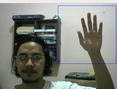
\includegraphics[width=0.5\linewidth]{recoghand}
	\caption{Ilustrasi Pengujian Pengenalan Gestur Tangan}
	\label{fig:recoghand}
\end{figure}
Ilustrasi pengujian ini digambarkan pada Gambar 4.10. Pengujian pengenalan gestur tangan dilakukan secara manual dan terpisah dari deteksi tangan, tahap ini memiliki perlakuan sama dengan tahap sebelumnya, yaitu menggunakan 3 subjek yang berbeda, kemudian dilakukan pengenalan gestur tangan sebanyak 10 kali untuk setiap klasifikasi. Total citra yang didapat dalam satu kondisi lux oleh satu subjek adalah 100 citra.
Tahap berikutnya dilakukan penurunan intensitas cahaya, dengan mengatur cahaya lampu di ruangan uji sebesar 50\% lux menggunakan dimmer. Pengujian dilakukan hingga batas lux kurang dari atau sama dengan 50 lux. Evaluasi yang dilakukan dengan \emph{confussion matrix} menggunakan data yang diperoleh pada Tabel 4.2. Hasil evaluasi pengujian akan diperoleh nilai akurasi untuk setiap kondisi lux. 
\begin{table}[H]
	\caption{Pengujian Pengenalan Gestur Tangan}
	\vspace{0cm}
	\centering
\begin{tabular}{|c|}
	\hline
	\multicolumn{1}{|c|}{Nilai Lux(X)}\\

	\begin{tabular}{|c|c|c|c|c|c|c|c|c|c|c|c|c|c|c|c|c|c|c|c|c|c|c|c|c|c|c|c|c|c|c|c|c|}
		\hline
		Klasifikasi & \multicolumn{10}{|c|}{Pengenalan Subjek\_1}& \multicolumn{10}{|c|}{Pengenalan Subjek\_2}& \multicolumn{10}{|c|}{Pengenalan Subjek\_3}\\
		\hline Angka 0 & & & &&&&&&&&&&&&&&&&&&&&&&&&&&&\\
		\hline Angka 1 & & & &&&&&&&&&&&&&&&&&&&&&&&&&&&\\
		\hline Angka 2 & & & & && &&&&&&&&&&&&&&&&&&&&&&&&\\
		
		\hline ... & & & &&&&&&&&&&&&&&&&&&&&&&&&&&& \\
		\hline Angka 9 & & & &&&&&&&&&&&&&&&&&&&&&&&&&&& \\
		\hline
	\end{tabular}
\end{tabular}
%%======================================================
\begin{tabular}{|c|}
	\multicolumn{1}{|c|}{Nilai Lux(...)}\\	
	\begin{tabular}{|c|c|c|c|c|c|c|c|c|c|c|c|c|c|c|c|c|c|c|c|c|c|c|c|c|c|c|c|c|c|c|c|c|}
		\hline
		Klasifikasi & \multicolumn{10}{|c|}{Pengenalan Subjek\_1}& \multicolumn{10}{|c|}{Pengenalan Subjek\_2}& \multicolumn{10}{|c|}{Pengenalan Subjek\_3}\\
		\hline Angka 0 & & & &&&&&&&&&&&&&&&&&&&&&&&&&&&\\
		\hline Angka 1 & & & &&&&&&&&&&&&&&&&&&&&&&&&&&&\\	
		\hline Angka 2 & & & &&&&&&&&&&&&&&&&&&&&&&&&&&&\\	
		\hline ... & & & &&&&&&&&&&&&&&&&&&&&&&&&&&& \\
		\hline Angka 9 & & & &&&&&&&&&&&&&&&&&&&&&&&&&&& \\
		\hline
	\end{tabular}	
\end{tabular}
%%======================================================
\begin{tabular}{|c|}

	\multicolumn{1}{|c|}{Nilai Lux(X$\le$50)}\\
	\begin{tabular}{|c|c|c|c|c|c|c|c|c|c|c|c|c|c|c|c|c|c|c|c|c|c|c|c|c|c|c|c|c|c|c|c|c|}
		\hline
		Klasifikasi & \multicolumn{10}{|c|}{Pengenalan Subjek\_1}& \multicolumn{10}{|c|}{Pengenalan Subjek\_2}& \multicolumn{10}{|c|}{Pengenalan Subjek\_3}\\
		\hline Angka 0 & & & &&&&&&&&&&&&&&&&&&&&&&&&&&&\\
		\hline Angka 1 & & & &&&&&&&&&&&&&&&&&&&&&&&&&&&\\	
		\hline Angka 2 & & & &&&&&&&&&&&&&&&&&&&&&&&&&&&\\
		\hline ... & & & &&&&&&&&&&&&&&&&&&&&&&&&&&& \\
		\hline Angka 9 & & & &&&&&&&&&&&&&&&&&&&&&&&&&&& \\
		\hline
	\end{tabular}
\end{tabular}
\end{table}
\subsection{Pengujian Sistem Keseluruhan}
Pengujian tahap terakhir adalah pengujian keseluruhan sistem yang dilakukan secara manual, dengan menggabungkan \emph{retinex}, deteksi tangan dan pengenalan gestur tangan dalam satu program utuh. Pengenalan akan terjadi apabila sebuah tangan dideteksi terlebih dahulu, jika tidak terdeteksi maka tidak akan dilakukan pengenalan. Nilai yang didapatkan dari hasil pengujian ini berupa \emph{true positive} dan \emph{false positive}. \emph{True positive} didapatkan ketika sebuah \emph{input} citra gestur dari webcam menghasilkan klasifikasi ASL yang sama dengan gestur ASL yang sebenarnya. Nilai \emph{false positive} terjadi apabila \emph{input} citra gestur dari webcam menghasilkan klasifikasi yang tidak sesuai dengan gestur ASL yang sebenarnya.

Penurunan intensitas dilakukan sama seperti pengujian sebelumnya. Tabel pengujian yang digunakan mengacu pada Tabel 4.2. Evaluasi dari akurasi sistem keseluruhan dapat diperoleh menggunakan \emph{confusion matrix} pada data yang dicatat pada tabel. Nilai akurasi dihitung untuk setiap kondisi lux yang tercatat pada tabel pengujian.
\chapter{JADWAL PENELITIAN}
\begin{table}[htpb]
	\caption{Jadwal Penelitian}
	\vspace{0.2cm}
	\centering
	\begin{tabular}{|p{0.5cm}|p{4cm}|p{4cm}|p{4cm}|}
		\hline
		No & Kegiatan & Target & Waktu Penelitian \\
		\hline
		1 & Studi literatur & Menyelesaikan riview literature terkait dengan penelitian yang relevan & Oktober - Januari \\ 
		\hline
		2 & Pengumpulan Data & Mengumpulkan dataset gestur jari tangan & Maret  – April 2020\\
		\hline
		3 & Perancangan Model & Melakukan uji coba dan perancangan model Neural network dalam sistem untuk training data & Maret – Juni 2020 \\
		\hline
		4 & Implementasi & Melakukan training data untuk menghasilkan model & Juni – Agustus 2020 \\
		\hline
		5 & Pengujian & Menguji model secara realtime & Agustus – Oktober 2020 \\
		\hline
		6 & Penulisan  Laporan & Menyusun laporan secara bertahap & Maret – Desember 2020\\
		\hline
		
	\end{tabular}
\end{table}

%-----------------------------------------------------------------
%Disini akhir masukan Bab
%-----------------------------------------------------------------

%-----------------------------------------------------------------
%Disini awal masukan untuk Daftar Pustaka (ISI SESUAI DENGAN DATA ANDA!)
%-----------------------------------------------------------------
\begin{thebibliography}{99}
\setlength\itemindent{-30pt}\singlespacing\addcontentsline{toc}{chapter}{DAFTAR PUSTAKA}

\bibitem[Aribowo(2009)]{ari}
Aribowo, E., Yustina, E., Studi, P., Informatika, T., Teknologi, F., Universitas, I. 
\& Dahlan, A., 2009, \emph{Implementasi Metode Retinex Untuk Pencerahan Citra}, 
Jurnal Informatika, 3, 2, 323–330. 

\bibitem[Loh(2019)]{loh}
Loh, Y.P., Liang, X. \& Chan, C.S., 2019,\emph{Low-light image enhancement using Gaussian Process for features retrieval}, Signal Processing: Image 
Communication, 74, 175–190. https://doi.org/10.1016/j.image.2019.02.001,. 

\bibitem[Saputra(2016)]{sap}
Saputra, L.K.P., 2016, \emph{Perbandingan Varian Metode Multiscale Retinex Untuk Peningkatan Akurasi Deteksi Wajah Adaboost HAAR-like}, Jurnal Teknik Informatika dan Sistem Informasi, 2, 1, 89–98.

\bibitem[Shen(2017)]{shen}
Shen, L., Yue, Z., Feng, F., Chen, Q., Liu, S. \& Ma, J., 2017, \emph{MSR-net:Low-light 
Image Enhancement Using Deep Convolutional Network}, , , January. 
http://arxiv.org/abs/1711.02488,.

\bibitem[Tanaka(2017)]{tan}
Tanaka, Y., Yamashita, Y., Nishikawa, K., Yamaguchi, T. \& Nishitani, T., 2019,\emph{Retinex Foreground Segmentation for Low Light Environments}, 2018 Asia-Pacific Signal and Information Processing Association Annual Summit and
Conference, APSIPA ASC 2018 - Proceedings, , November, 285–290.

\bibitem[Yingx(2017)]{yin}
Yingxin, X., Jinghua, L., Lichun, W. \& Dehui, K., 2017,\emph{A Robust Hand Gesture Recognition Method via Convolutional Neural Network}, Proceedings - 2016 
International Conference on Digital Home, ICDH 2016, 64–67. 

\bibitem[Sarifudin(2015)]{sar}
Madenda,Sarifudin., 2015, \emph{Pengolahan \& Video Digital}, Erlangga, 
Jakarta[BUKU].

\bibitem[Neilsen(2015)]{neil}
Nielsen, M., 2015, \emph{Neural Networks and Deep Learning, Determination Press}., 
[Daring]. tersedia di \emph{http://neuralnetworksanddeeplearning.com}. 

\bibitem[Munir(2004)]{mun}
Rinaldi, Munir., 2004, \emph{Pengolahan Citra Digital}, Bandung, Informatika[BUKU]. 

\bibitem[hidayatullah(2017)]{hid}
Hidayatullah, Priyanto,. 2017,\emph{Pengolahan Citra Digital Teori dan Aplikasi Nyata}, 
Bandung, Informatika[BUKU].

\bibitem[barczak(2011)]{bar}
Barczak, A.L.C., Reyes, N.H., Abastillas, M., Piccio, A. \& Susnjak, T., 2011, \emph{A New 2D Static Hand Gesture Colour Image Dataset for ASL Gestures},Res. Lett. Inf. Math. Sci., 15, 12-20.\emph{http://iims.massey.ac.nz/research/letters/}.

\bibitem[kolkur(2017)]{kol}
Kolkur, S., Kalbande, D., Shimpi, P., Bapat, C. \& Jatakia, J., 2017, \emph{Human Skin Detection Using RGB , HSV and YCbCr Color Models}, , 137, 324-332.

\bibitem[arabi(2019)]{arb}
Arabi, S., Haghighat, A. \& Sharma, A., 2019, \emph{A deep learning based solution for construction equipment detection: from development to deployment} , , , April.

\bibitem[srinivan(2016)]{sri}
Srinivasan, R., 2016, \emph{Implementing Histogram Equalization and Retinex}, , , July.

\bibitem[huang(2019)]{hua}
Huang, H., Chong, Y., Nie, C. \& Pan, S., 2019, \emph{Hand Gesture Recognition with Skin Detection and Deep Learning Method Hand Gesture Recognition with Skin Detection and Deep Learning Method}, J. Phys.: Conf. Ser. 1213 022001.

\bibitem[Posada(2007)]{pos}
Posada-Gómez, Rubén \& Sanchez Medel, Luis \& Alor-Hernández, Giner \& Martinez Sibaja, Albino \& Aguilar-Laserre, A. \& Leija-Salas, L.. 2007. \emph{A Hands Gesture System Of Control For An Intelligent Wheelchair}. 68 - 71. 10.1109/ICEEE.2007.4344975. 

\bibitem[kemenkes(2015)]{kem}
Kemenkes, 2018, \emph{Indonesia Inklusi  dan Ramah Disabilitas}[Daring], tersedia di \emph{https://www.kemkes.go.id/resources/download/pusdatin/infodatin/infodatin-disabilitas.pdf}.

\bibitem[arfianto(2016)]{arf}
Afrianto, T. \& Amalia, F., 2016, \emph{Pengaruh Komponen Krominan Pada Ruang Warna}, Prosiding Seminar Nasional Teknologi Terapan (SNTT), August 2017, 282-285.

\bibitem[Howard(2017)]{how}
Howard, A.G., Zhu, M., Chen, B., Kalenichenko, D., Wang, W., Weyand, T., Andreetto, M. \& Adam, H., 2017, \emph{MobileNets: Efficient Convolutional Neural Networks for Mobile Vision Applications}, \emph{http://arxiv.org/abs/1704.04861}.

\bibitem[Sandler(2018)]{sand}
Sandler, M., Howard, A., Zhu, M., Zhmoginov, A. \& Chen, L.C., 2018, \emph{MobileNetV2: Inverted Residuals and Linear Bottlenecks}, Proceedings of the IEEE Computer Society Conference on Computer Vision and Pattern Recognition, 45104520.

\bibitem[Google(2018)]{goog}
Google AI Blog., 2018, \emph{MobileNetV2: The Next Generation of On-Device Computer Vision Networks}[Daring], tersedia di \emph{ai.googleblog.com/2018/04/mobilenetv2-next-generation-of-on.html?m=1}.
\bibitem[Leonard(2017)]{Leo}
Leonard, L.C., 2017, \emph{Web-Based Behavioral Modeling for Continuous User 
	Authentication (CUA)}, 1 edisi, Elsevier Inc., [Daring]. tersedia di 
DOI:10.1016/bs.adcom.2016.12.001.
\bibitem[Hui(2018)]{hui}
Hui, Jonathan., 2018, \emph{mAP (mean Average Precision) for Object Detection}[Daring], tersedia di \emph{www.medium.com/@jonathan\_hui/map-mean-average-precision-for-object-detection-45c121a31173}.
\bibitem[Chen(2015) ]{chen}
Chen, X., Fang, H., Lin, T.Y., Vedantam, R., Gupta, S., Dollár, P \& Zitnick, C.L., 2015, \emph{Microsoft COCO Captions: Data Collection and Evaluation Server}, arXiv:1504.00325.
\bibitem[Petro(2014)]{Petro}
Petro., Ana-Belen \& Sbert., Catalina \& Morel., Jean-Michel., 2014. \emph{Multiscale Retinex}. Image Processing On Line, 4. 71-88, DOI:10.5201/ipol.2014.107. 
\bibitem[He(2016)]{He}
X. He., T. Wang., Y. Jia., Y. Wang., Z. Xie and D. Xie., 2016, \emph{Studying fidelity issues in image enhancement by means of multi-scale retinex with color restoration}, 2016 3rd International Conference on Systems and Informatics (ICSAI), Shanghai, pp. 536-540, DOI: 10.1109/ICSAI.2016.7811013.
\bibitem[Parihar(2018)]{Parihar}
A. S. Parihar and K. Singh., \emph{A study on Retinex based method for image enhancement}, 2018, 2nd International Conference on Inventive Systems and Control (ICISC), Coimbatore, pp. 619-624, DOI: 10.1109/ICISC.2018.8398874.
\end{thebibliography}

%-----------------------------------------------------------------
%-----------------------------------------------------------------


%-----------------------------------------------------------------
%Disini awal masukan untuk Lampiran (JIKA DIPERLUKAN)
%-----------------------------------------------------------------
\appendix
%\chapter{SKRIP}


%-----------------------------------------------------------------
%-----------------------------------------------------------------
\end{document}
